\subsection{Path-Planning with Reference Path}

\subsubsection{Algorithm}

%\begin{frame}{Coverage Model in Path-Planning}{Path-Planning with Reference Path}

%\begin{itemize}
%\item Information measurement - entropy 
%\item Maximum coverage problem
%\end{itemize}

%\begin{figure}
%\centering
%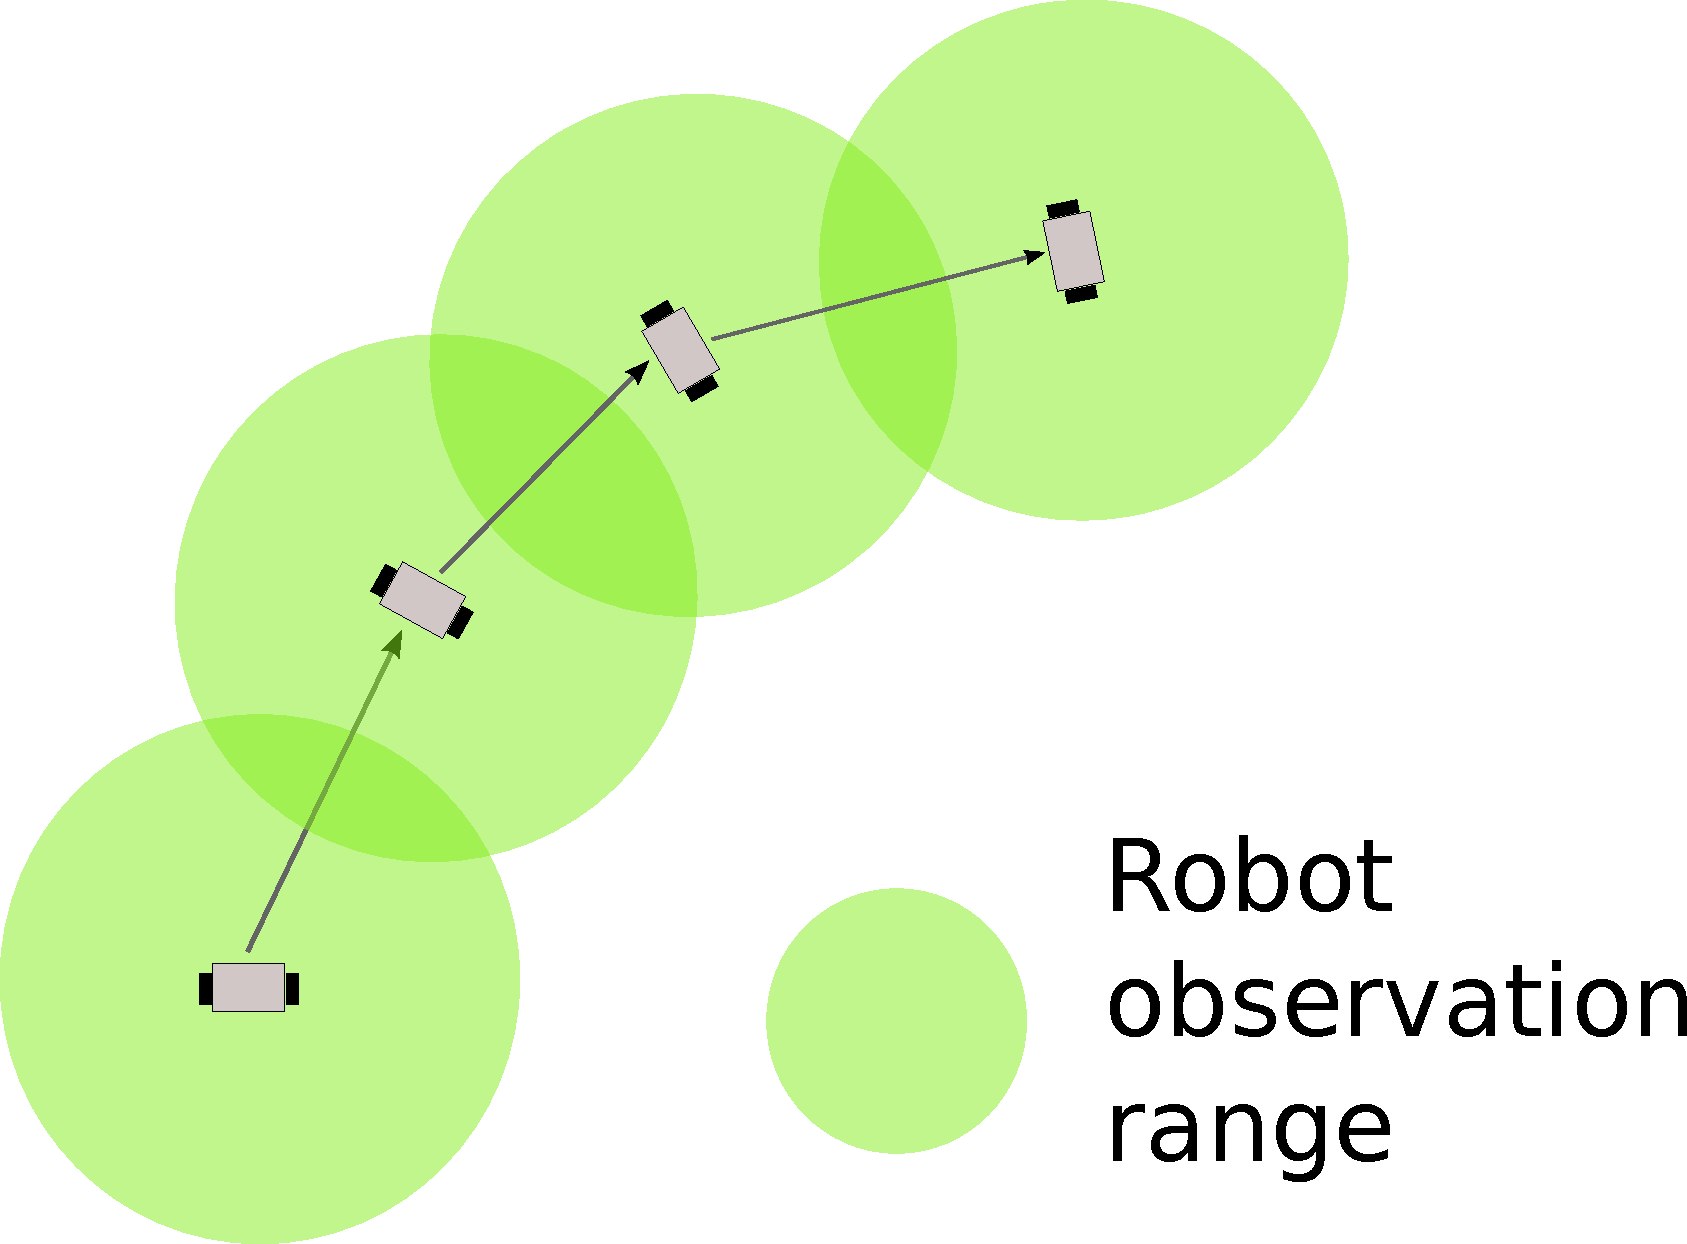
\includegraphics[width = 0.6\textwidth]{./figure/robotObservation}
%\end{figure}

%\end{frame}

\begin{comment}
\begin{frame}{Submodularity}{Path-Planning with Reference Path}

\begin{columns}

\column{0.45\textwidth}

\begin{figure}
\centering
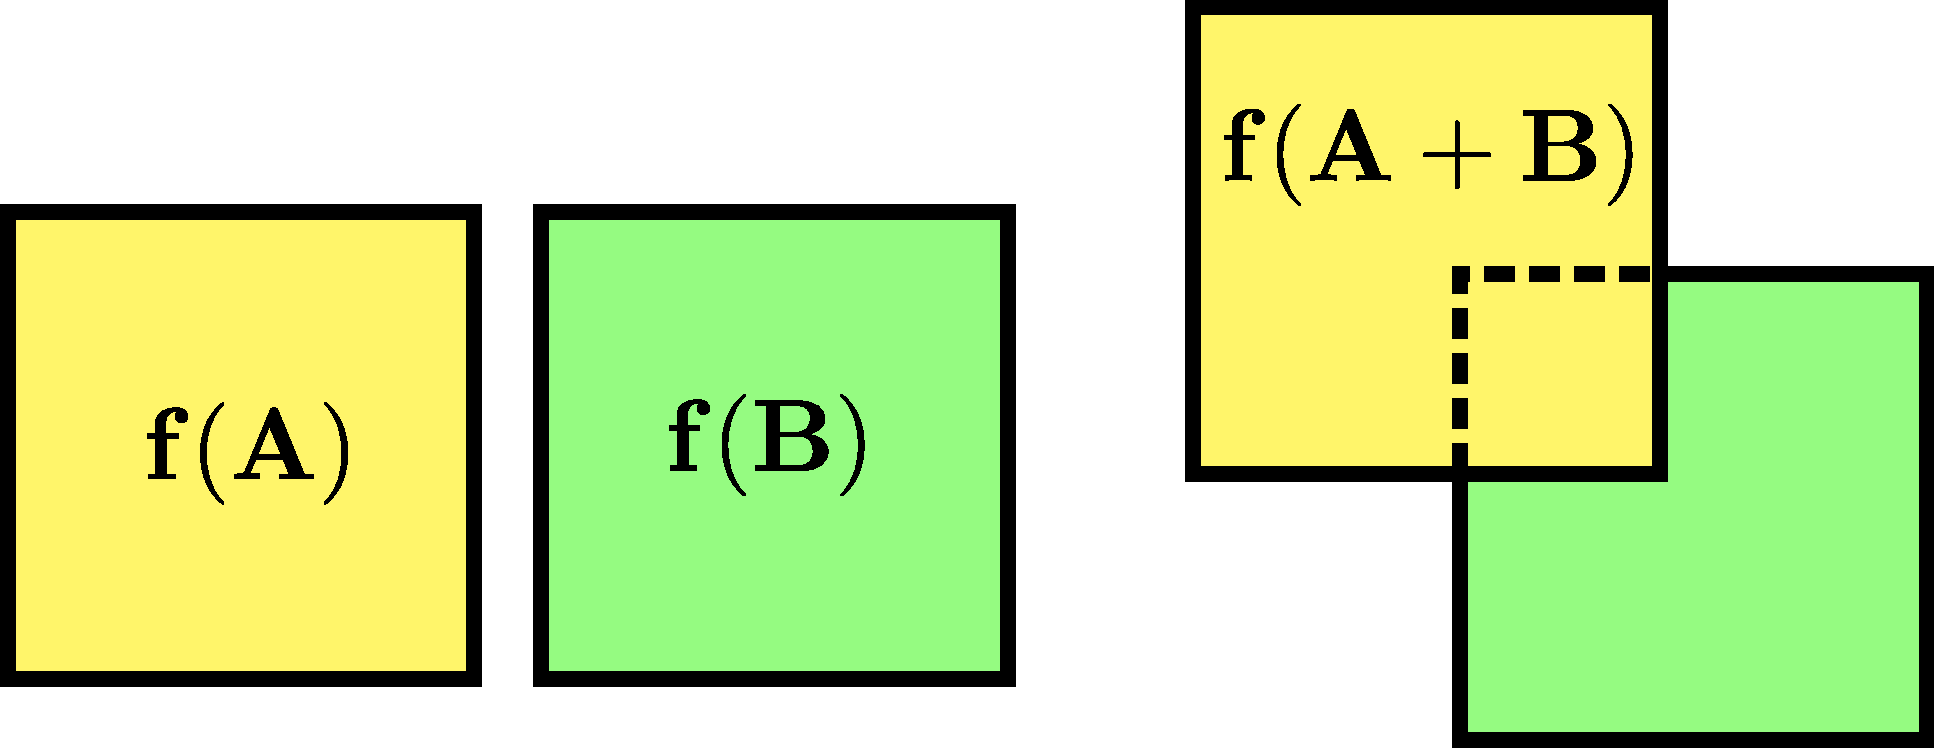
\includegraphics[width = \textwidth]{./figure/submodular}
%\caption{A coverage model.}
\end{figure}

\begin{equation}
\nonumber
f(A) + f(B) \geq f(A+B)
\end{equation}

\column{0.1\textwidth}

\column{0.45\textwidth}

Information
\begin{itemize}
\item search space $ S $
\item the observation of a robot $ \mathbf{O}^{X} $ 
\item the observation of a human $ \mathbf{O}^{Y} $

\bigskip
\bigskip

$ f( \mathbf{S}, \mathbf{O}^{X} ) + f( \mathbf{S}, \mathbf{O}^{Y^{h}} ) \geq f( \mathbf{S}, \mathbf{O}^{X},  \mathbf{O}^{Y^{h}} ) $ 
\end{itemize}

\end{columns}

\end{frame}

\begin{frame}{Submodular orienteering}{Path-Planning with Reference Path}

\begin{block}{Conditional mutual information}
$ I(\mathbf{S}; \mathbf{O}^{X} \mid \mathbf{O}^{Y^{h}}) = H(\mathbf{S} \mid \mathbf{O}^{Y^{h}}) - H(\mathbf{S} \mid \mathbf{O}^{X},\mathbf{O}^{Y^{h}}) $
\end{block} 

\bigskip

\begin{itemize}
\item Entropy reduction
\item Submodularity
\item Chain rule \\
$ I(\mathbf{S}; \mathbf{O}^{X} \mid \mathbf{O}^{Y^{h}}) = \sum_{t=1}^{T} I(O^{X}_{t} ; \mathbf{S} \mid O^{X}_{1} , \cdots , O^{X}_{t-1}, \mathbf{O}^{Y^{h}}) $
\end{itemize}

\end{frame}
\end{comment}

\begin{frame}{Human Constraint}{Path-Planning with Reference Path}

\begin{columns}
\column{.49\textwidth}
\begin{figure}
\centering
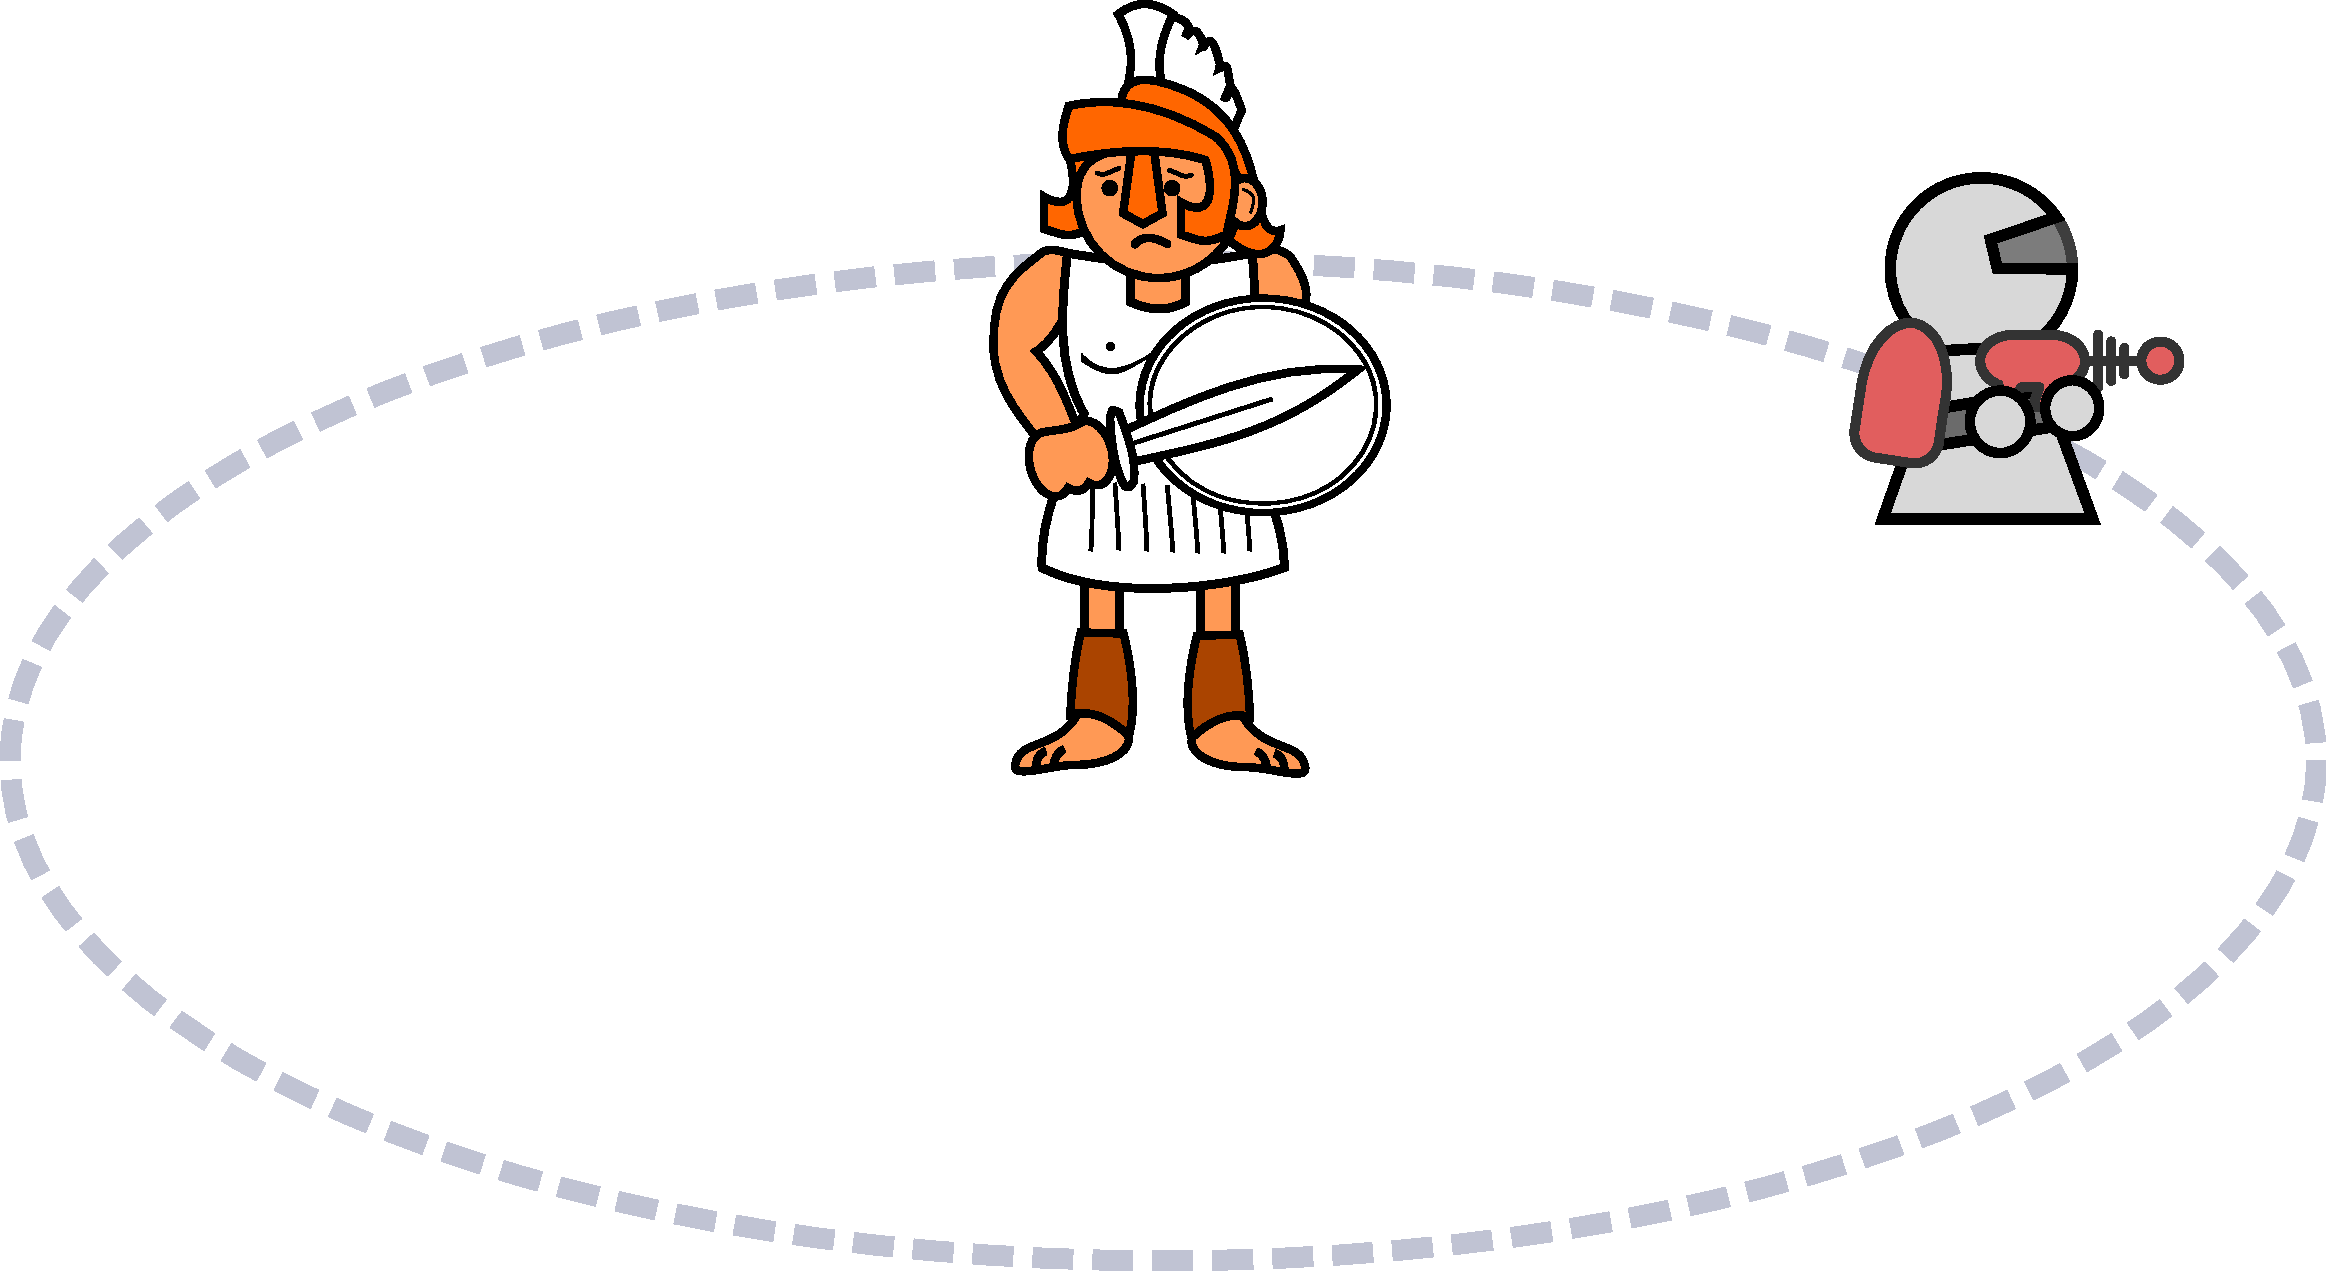
\includegraphics[width = \textwidth]{./figure/human_robot_interaction}
\end{figure}

\begin{itemize}
\item cooperative observation
\item assistance and protection
\end{itemize}

\column{.49\textwidth}
\begin{figure}
	\centering
	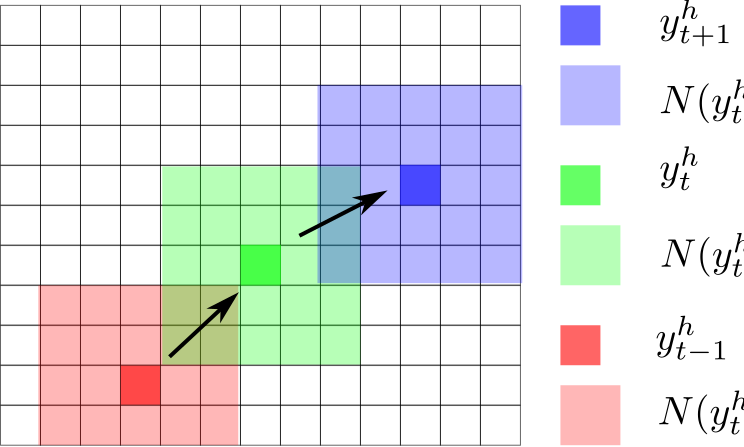
\includegraphics[width = \textwidth]{./figure/humanConstraint}
\end{figure}
\begin{itemize}
	\item { human path $ \{ y^{h}_{1} \cdots y^{h}_{T} \} $ }
	\item { neighboring function $ N( y^{h}_{t} ) $ }
\end{itemize}

\end{columns}

\end{frame}

\begin{frame}{Reference Path}{Path-Planning with Reference Path}

\begin{figure}
\centering
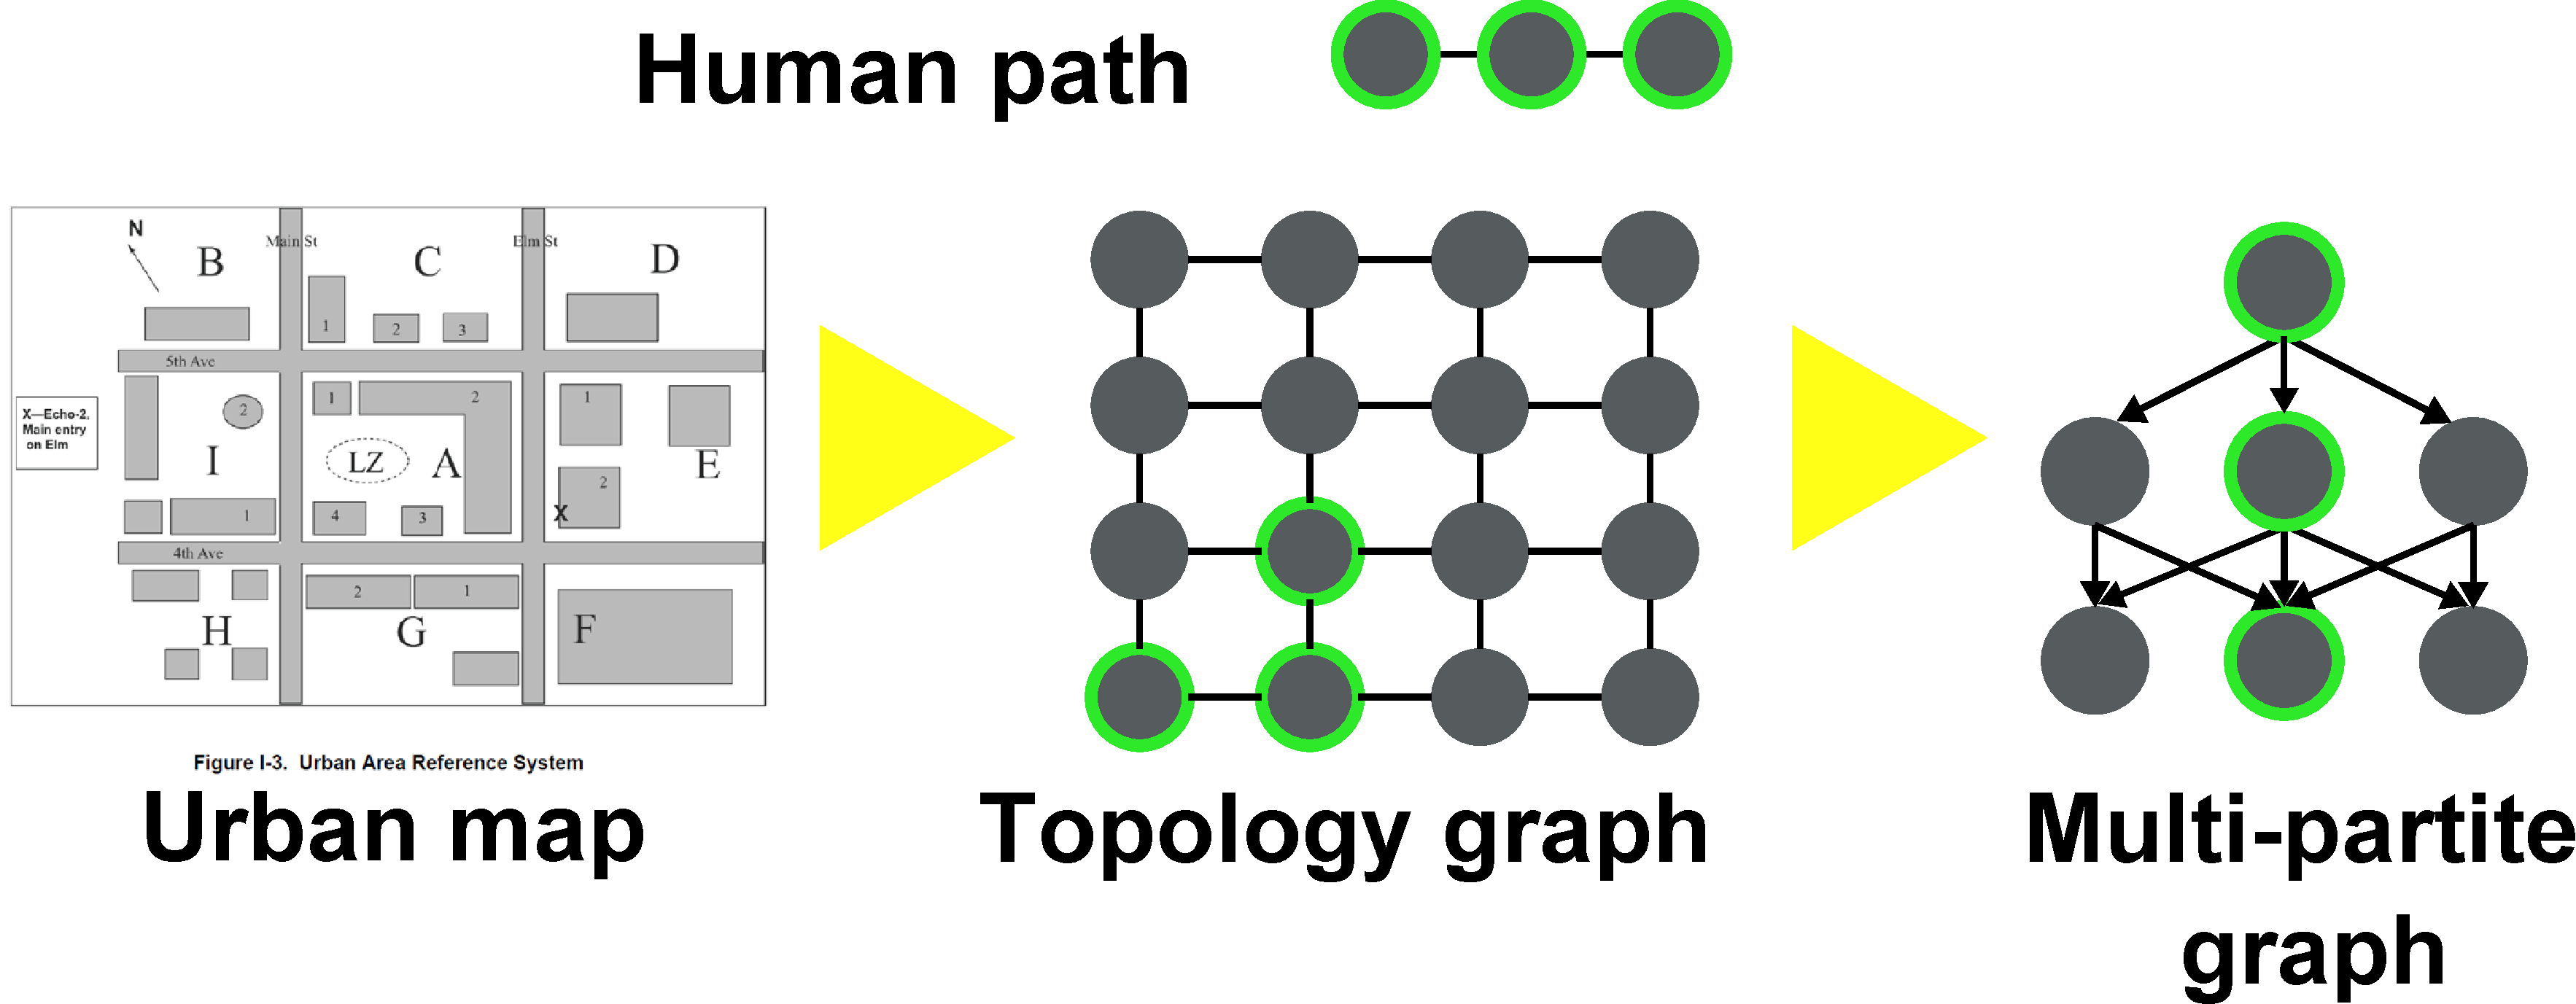
\includegraphics[width = 0.9\textwidth]{./figure/layers}
\end{figure}

\begin{figure}
	\centering
	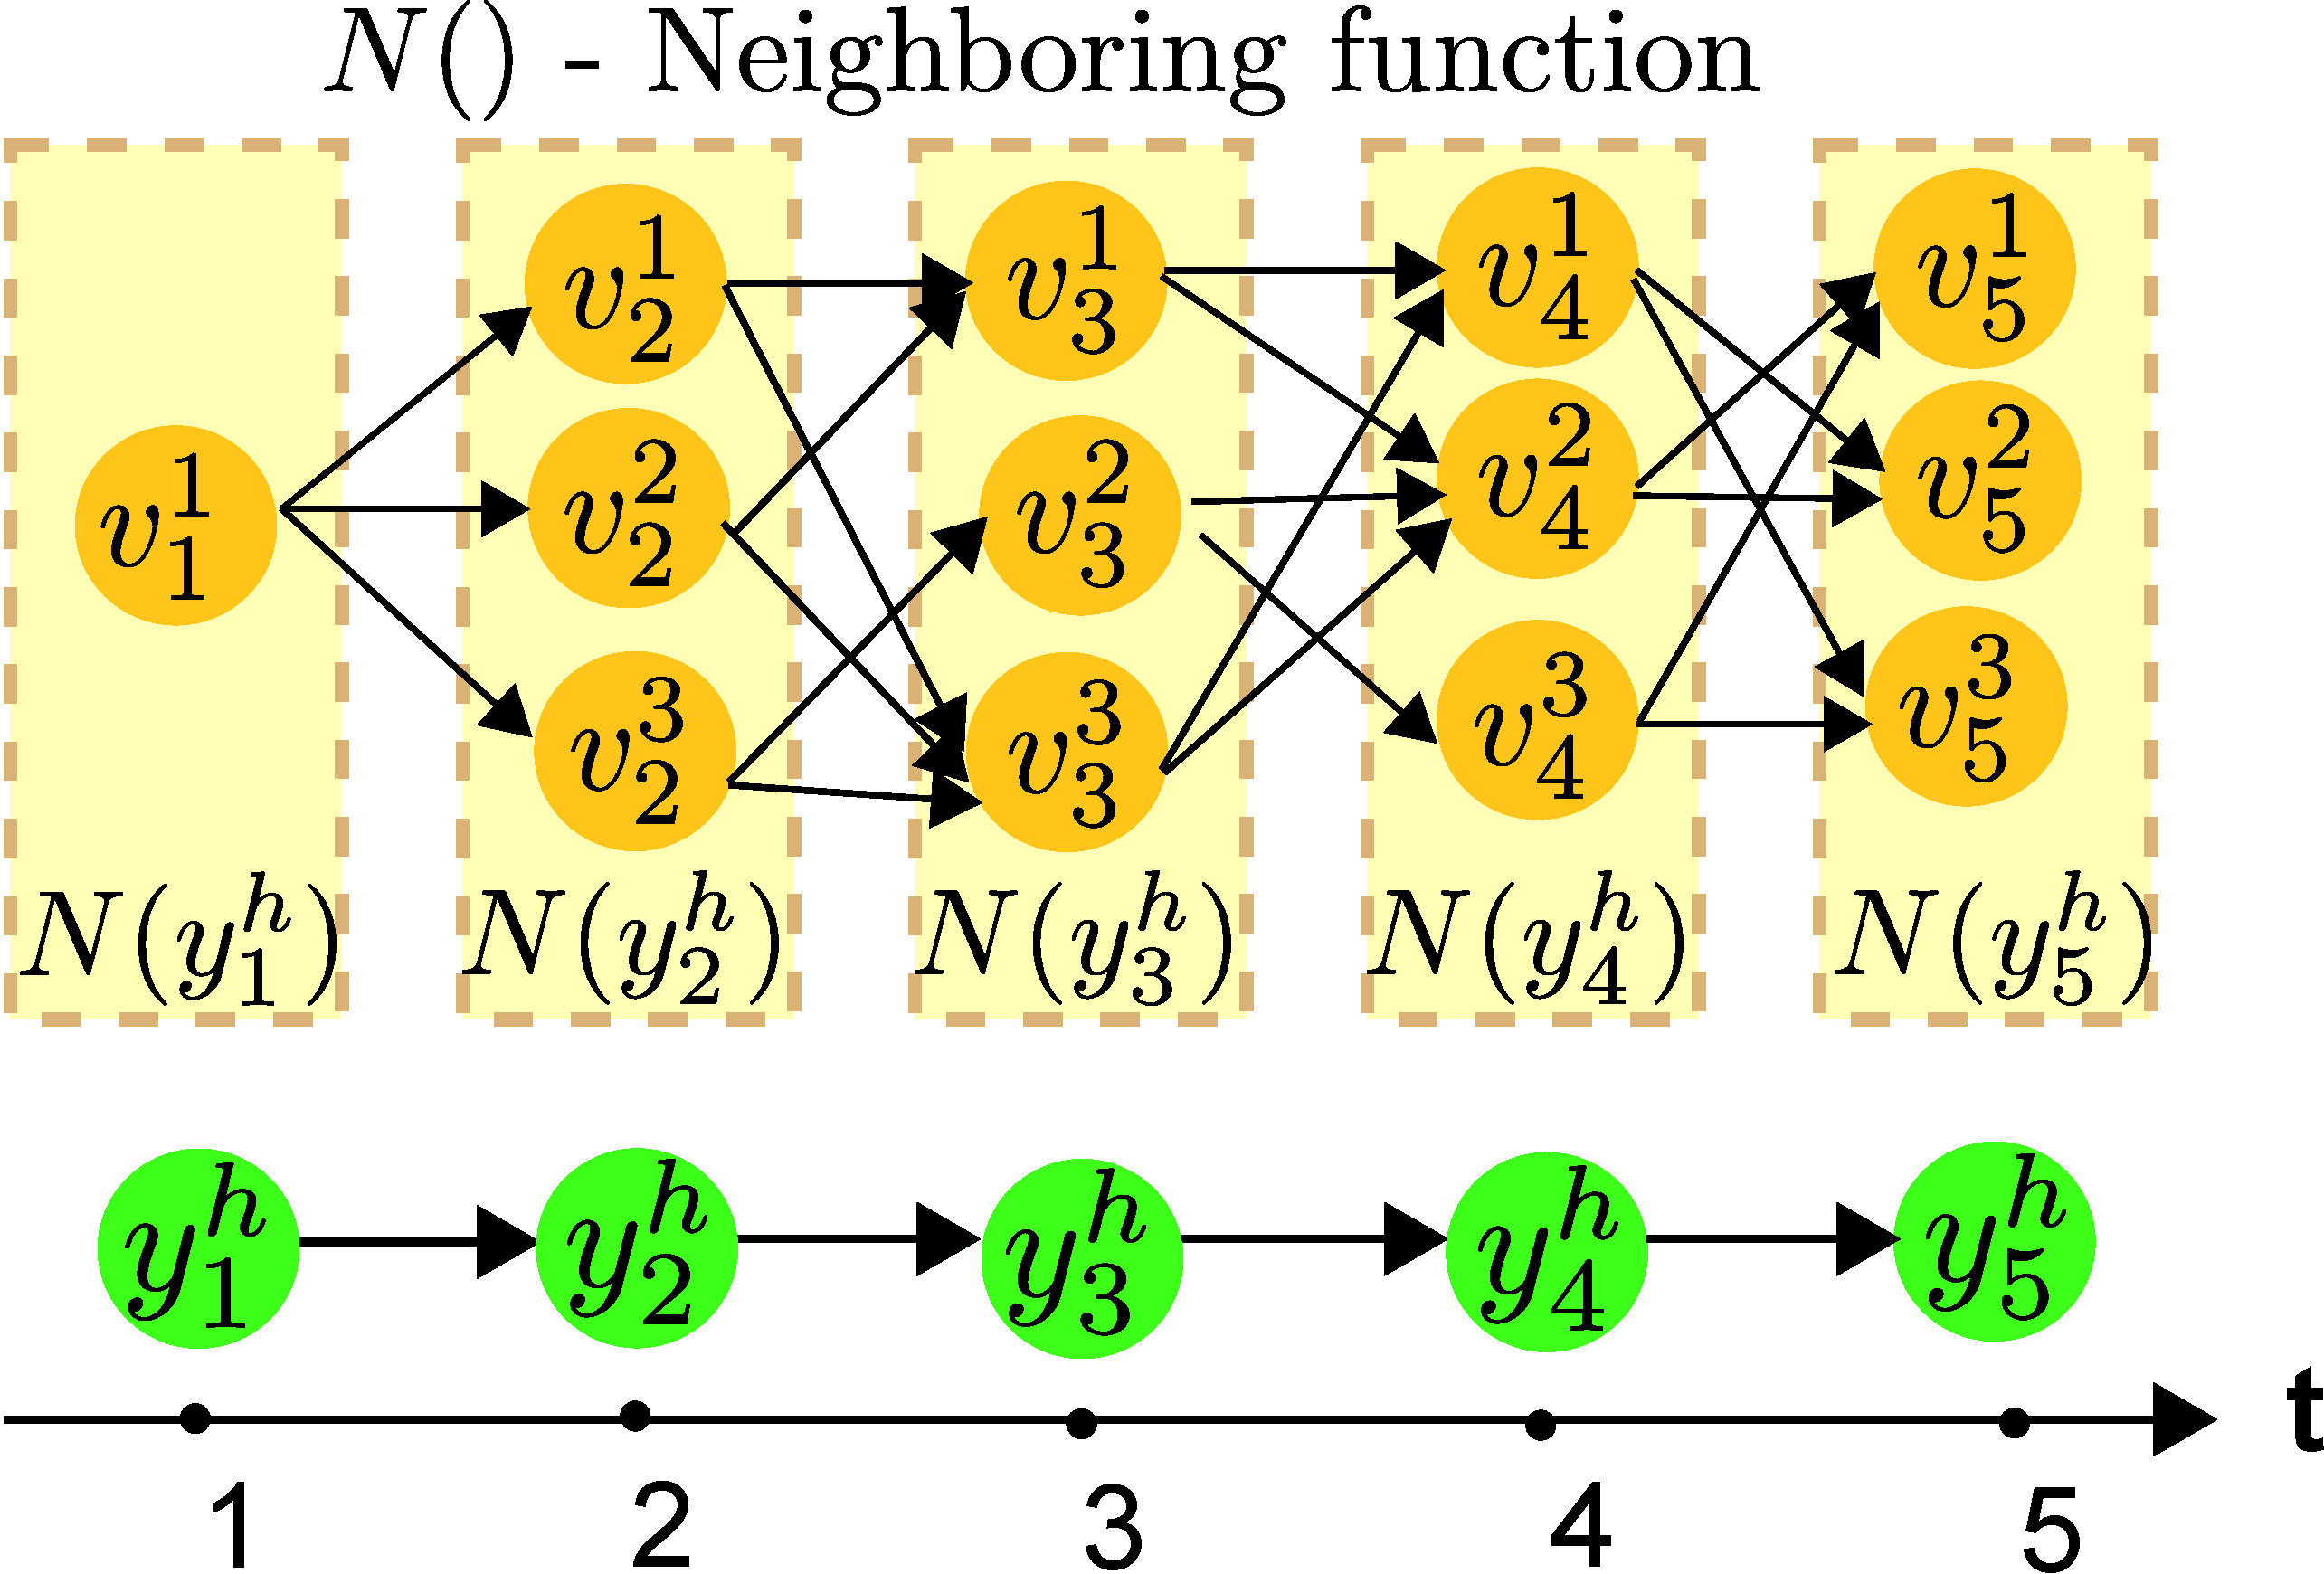
\includegraphics[width = .5\textwidth]{./figure/MultiPartite}
\end{figure}

\end{frame}

\begin{comment}
\begin{frame}{The Multi-Partite Graph}{Path-Planning with Reference Path}

\begin{columns}

\column{.6\textwidth}
\begin{minipage}[c]{\textwidth}
\begin{figure}
\centering
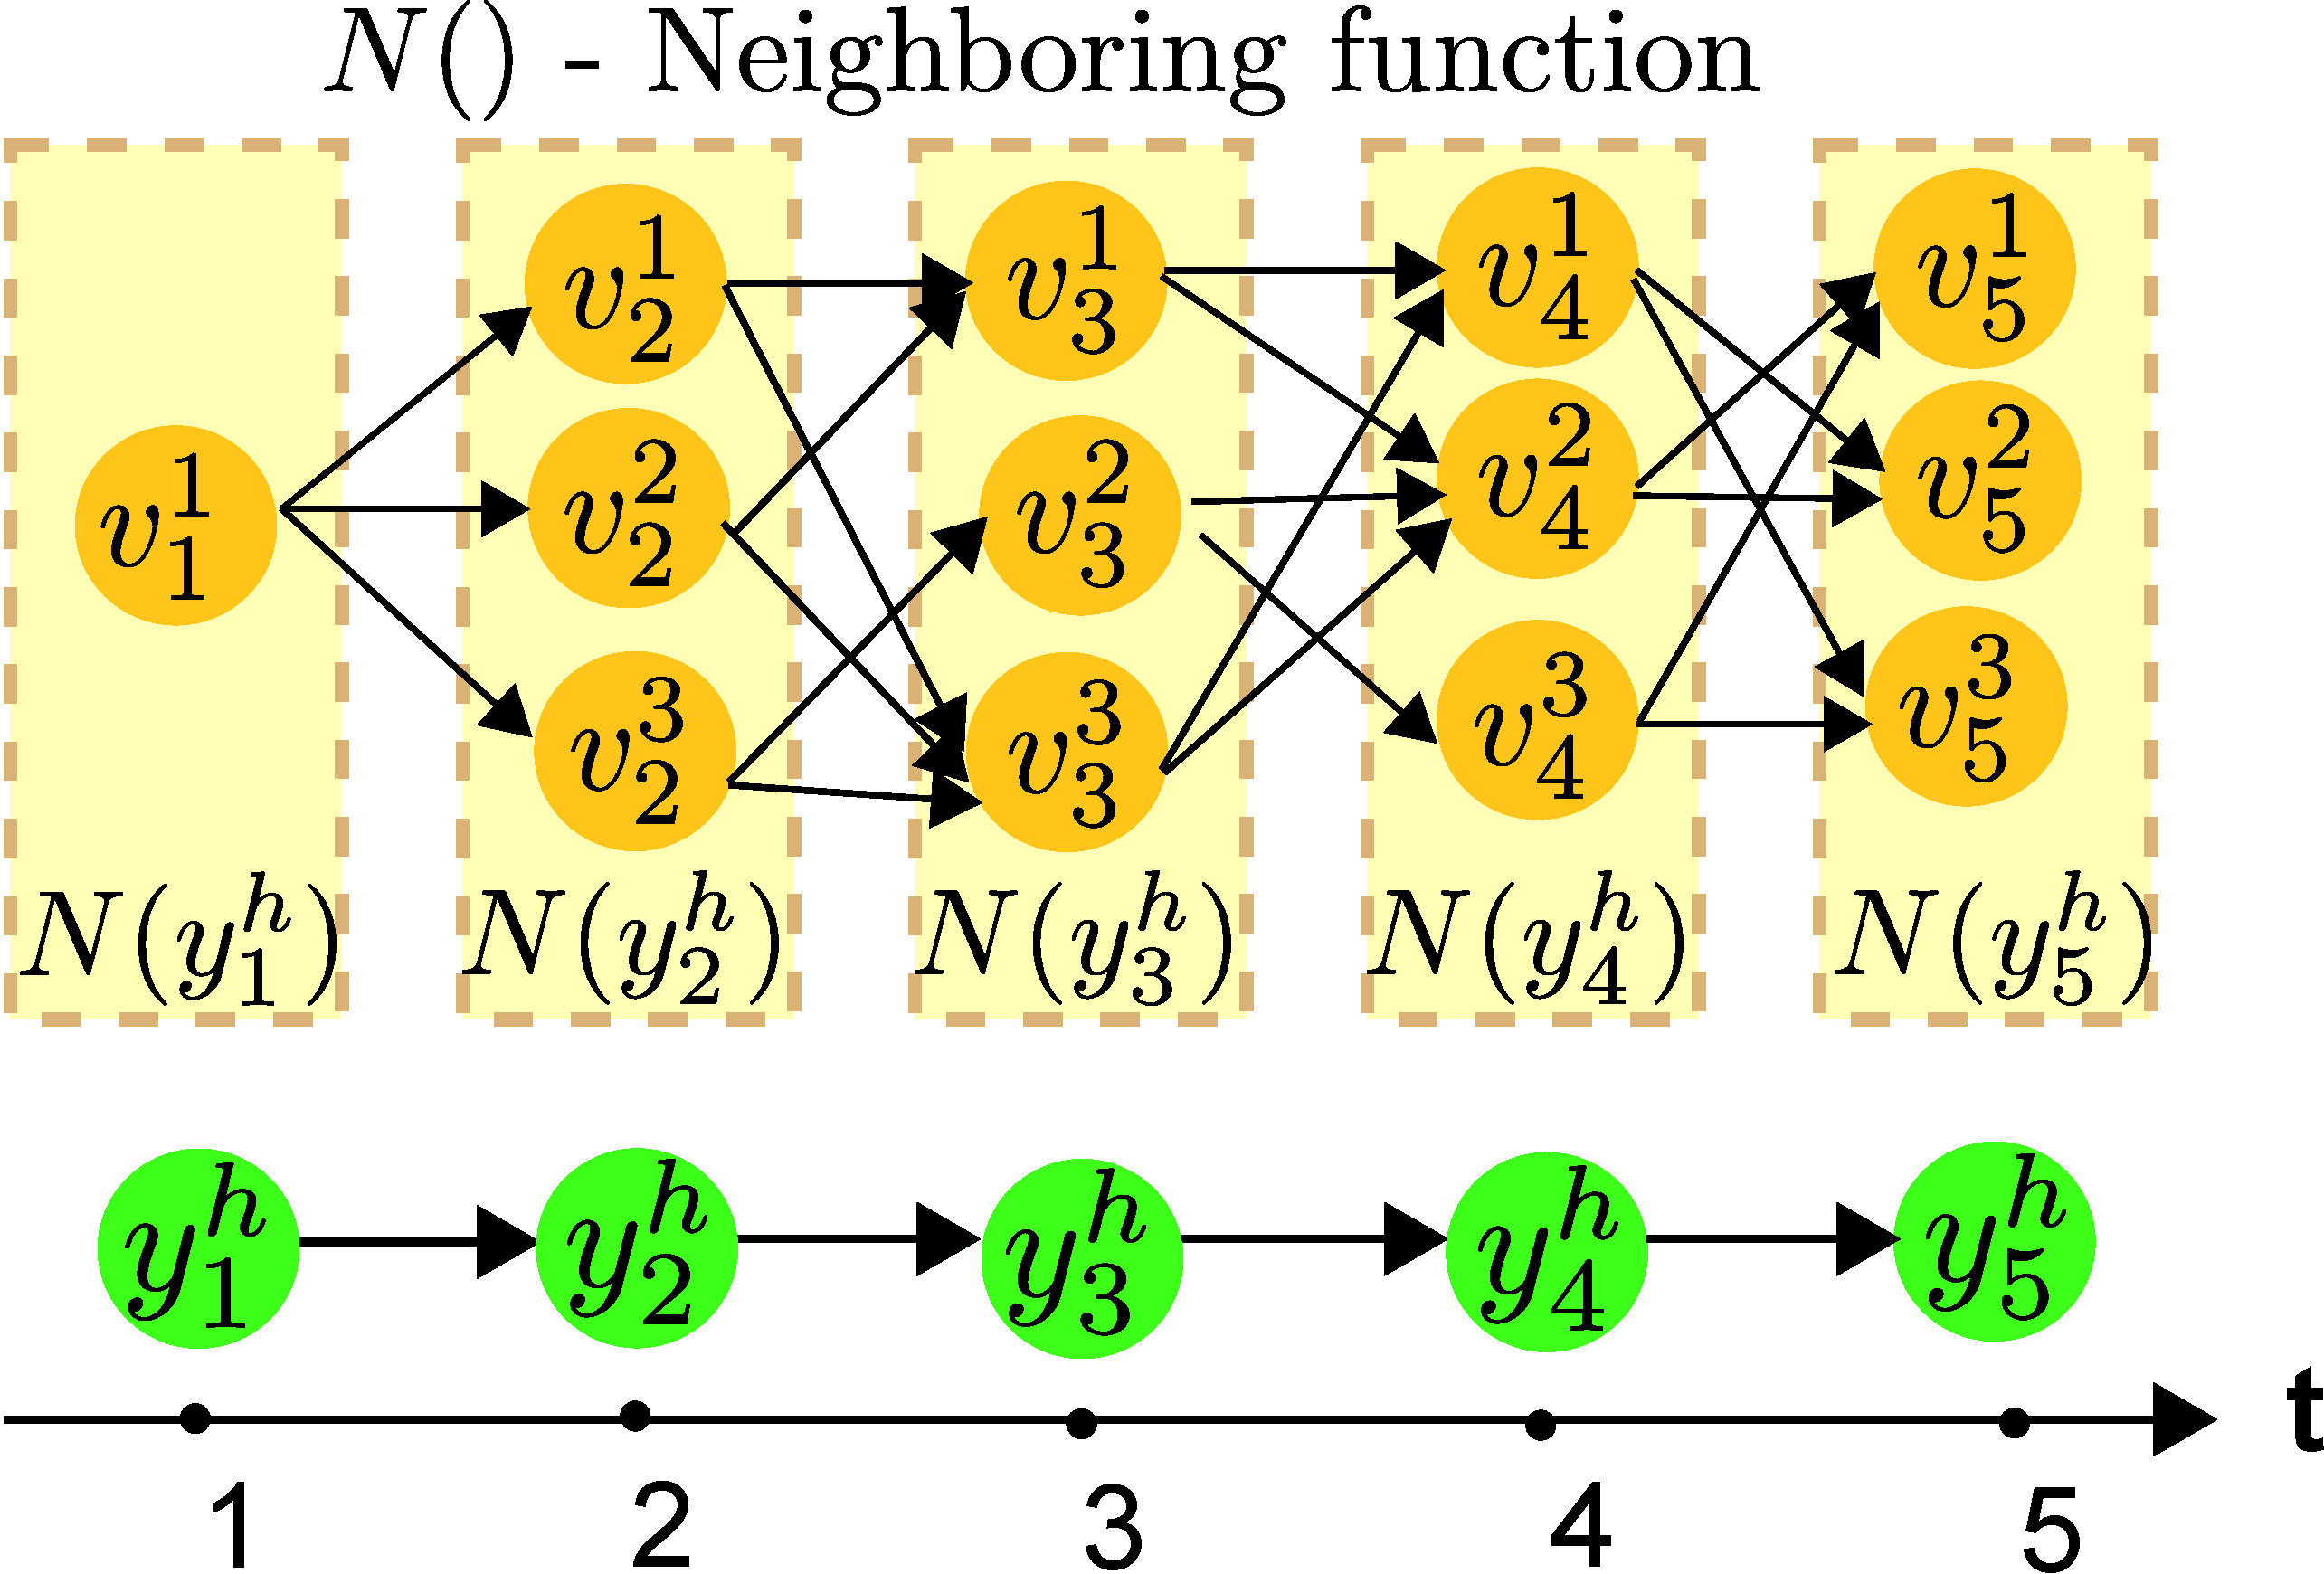
\includegraphics[width = .8\textwidth]{./figure/MultiPartite}
\end{figure}
\end{minipage}

\column{.4\textwidth}
\begin{minipage}[c]{\textwidth}
\begin{itemize}
\item time-space synchronization
\item connection determined by discretized map
\end{itemize}
\end{minipage}

\end{columns}

\begin{block}{Submodular Orienteering on a Multi-Partite Graph}
\begin{equation}
\nonumber
\begin{aligned}
Objective: & X^{*} = \argmax_{X} \: f(X); \\
Constraint: & |X| = T, x_{t} \in V(t), (x_{t}, x_{t+1}) \in E.
\end{aligned}
\end{equation}
\end{block}

\end{frame}
\end{comment}

\begin{frame}{A Pruning Process}{Path-Planning with Reference Path}

\begin{columns}

\column{.47\textwidth}
\begin{block}{Forward Pruning}
Reachable 
\begin{columns}
\column{.15\textwidth}
\column{.4\textwidth}
\tiny{
\noindent
$ \forall t \in \{ 2, \cdots T \}, $ \\
$ \forall v \in V(t), $  \\
$ deg^{-}(v) > 0 $
}
\column{.3\textwidth}
\begin{figure}
\centering
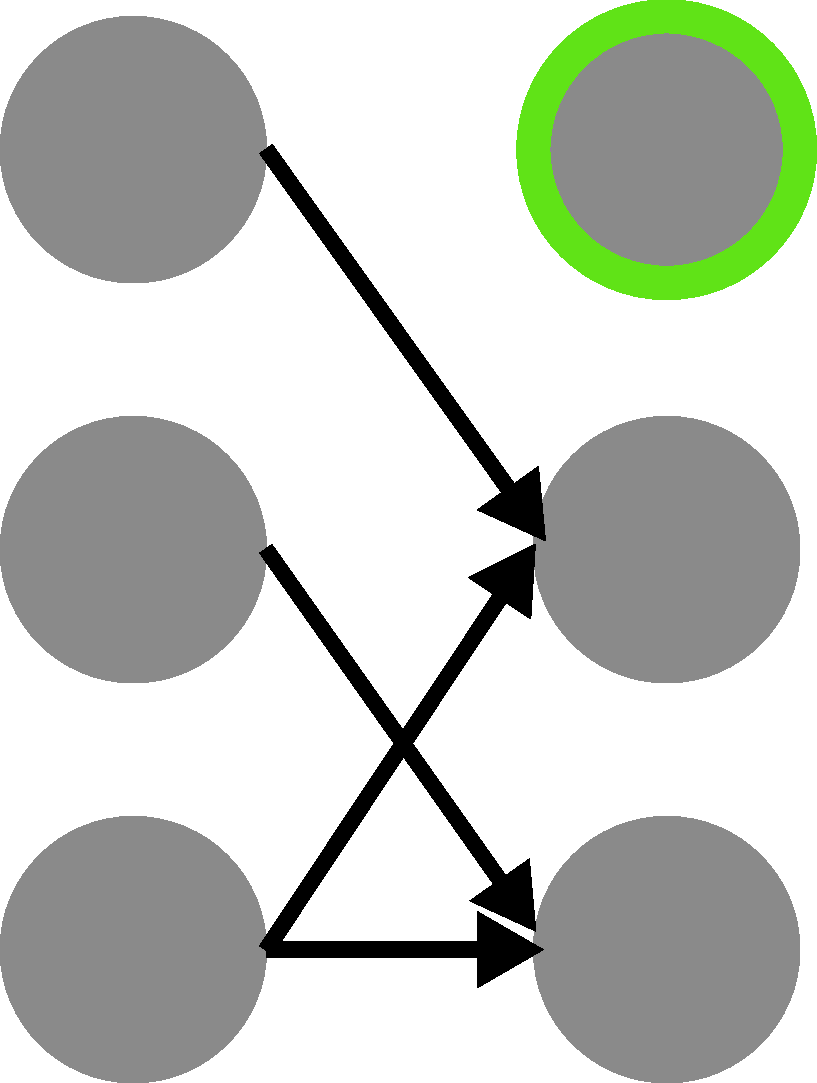
\includegraphics[width = \textwidth]{./figure/forward_prune}
\end{figure}
\column{.15\textwidth}
\end{columns}
\end{block}

\column{.47\textwidth}

\begin{block}{Backward Pruning}
Non-terminating 
\begin{columns}
\column{.15\textwidth}
\column{.4\textwidth}
\tiny{
\noindent
$ \forall t \in \{ 1, \cdots T-1 \}, $ \\
$ \forall v \in V(t), $ \\ 
$ deg^{+}(v) > 0 $
}
\column{.3\textwidth}
\begin{figure}
\centering
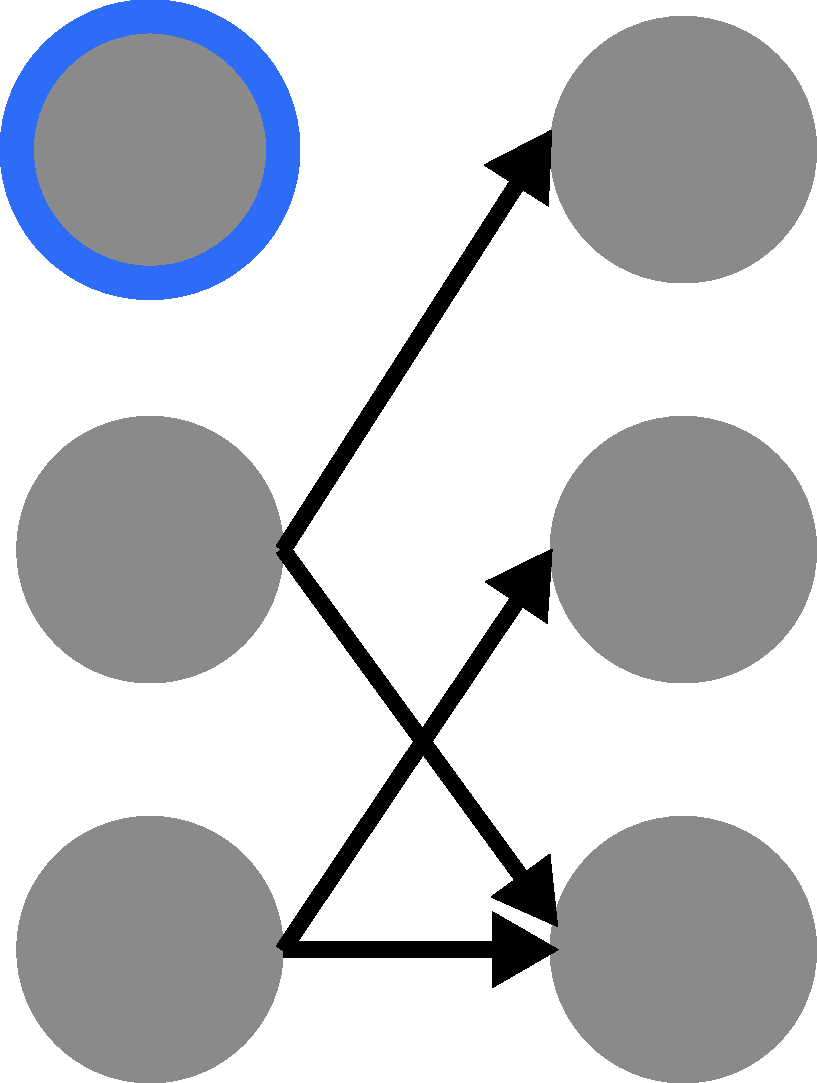
\includegraphics[width = \textwidth]{./figure/backward_prune}
\end{figure}
\column{.15\textwidth}
\end{columns}
\end{block}

\end{columns}

\begin{block}{Obstacles}
\begin{figure}
\centering
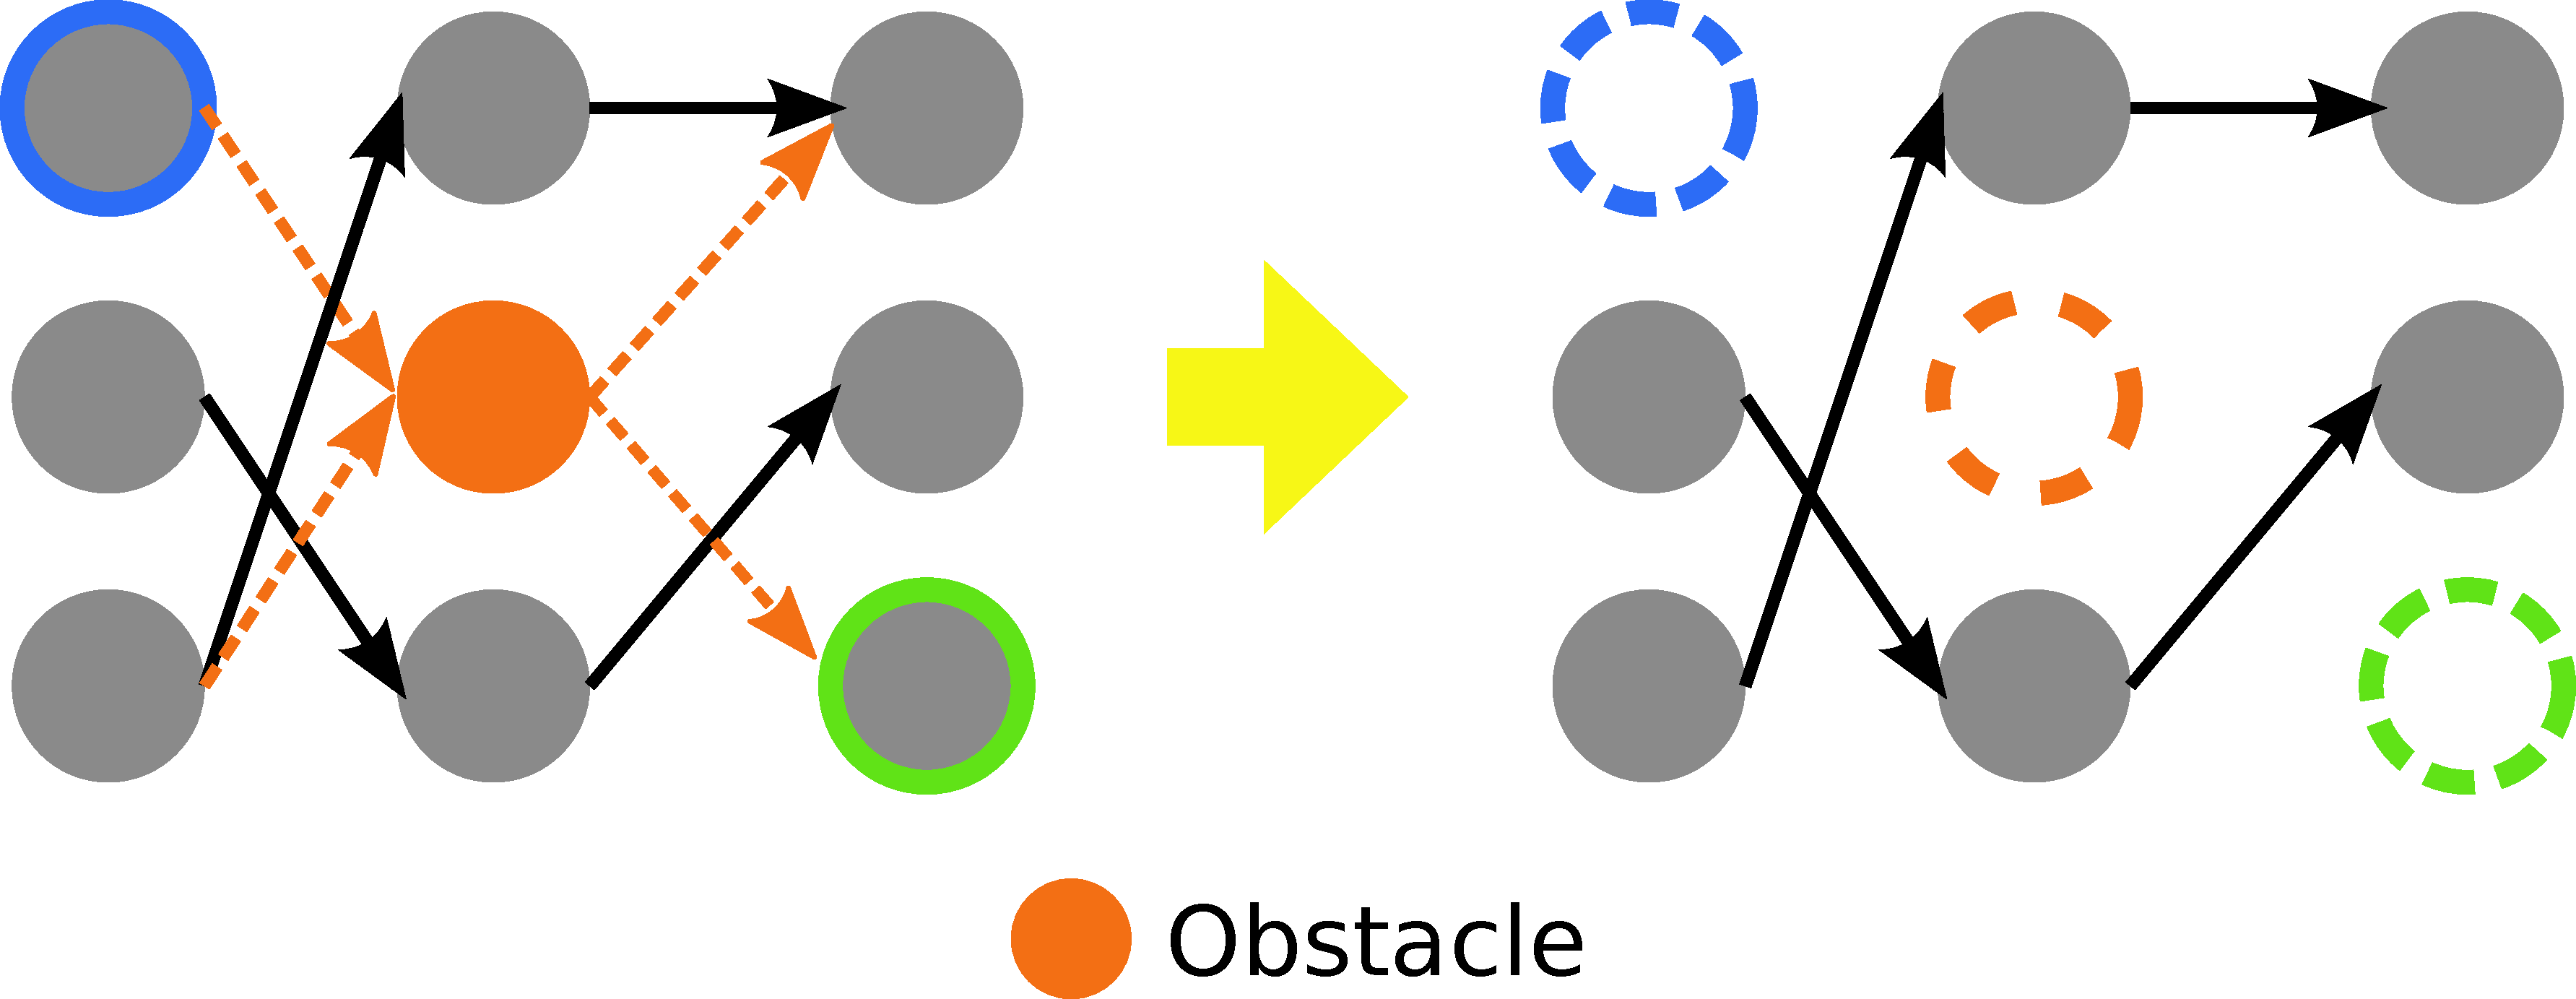
\includegraphics[width = 0.5\textwidth]{./figure/obstacle}
\end{figure}
\end{block}

\end{frame}

\begin{frame}{Algorithms}{Path-Planning with Reference Path}

\begin{columns}

\column{0.5\textwidth}
\begin{minipage}{\textwidth}
\begin{block}{Backtracking Heuristic}
\begin{figure}
\centering
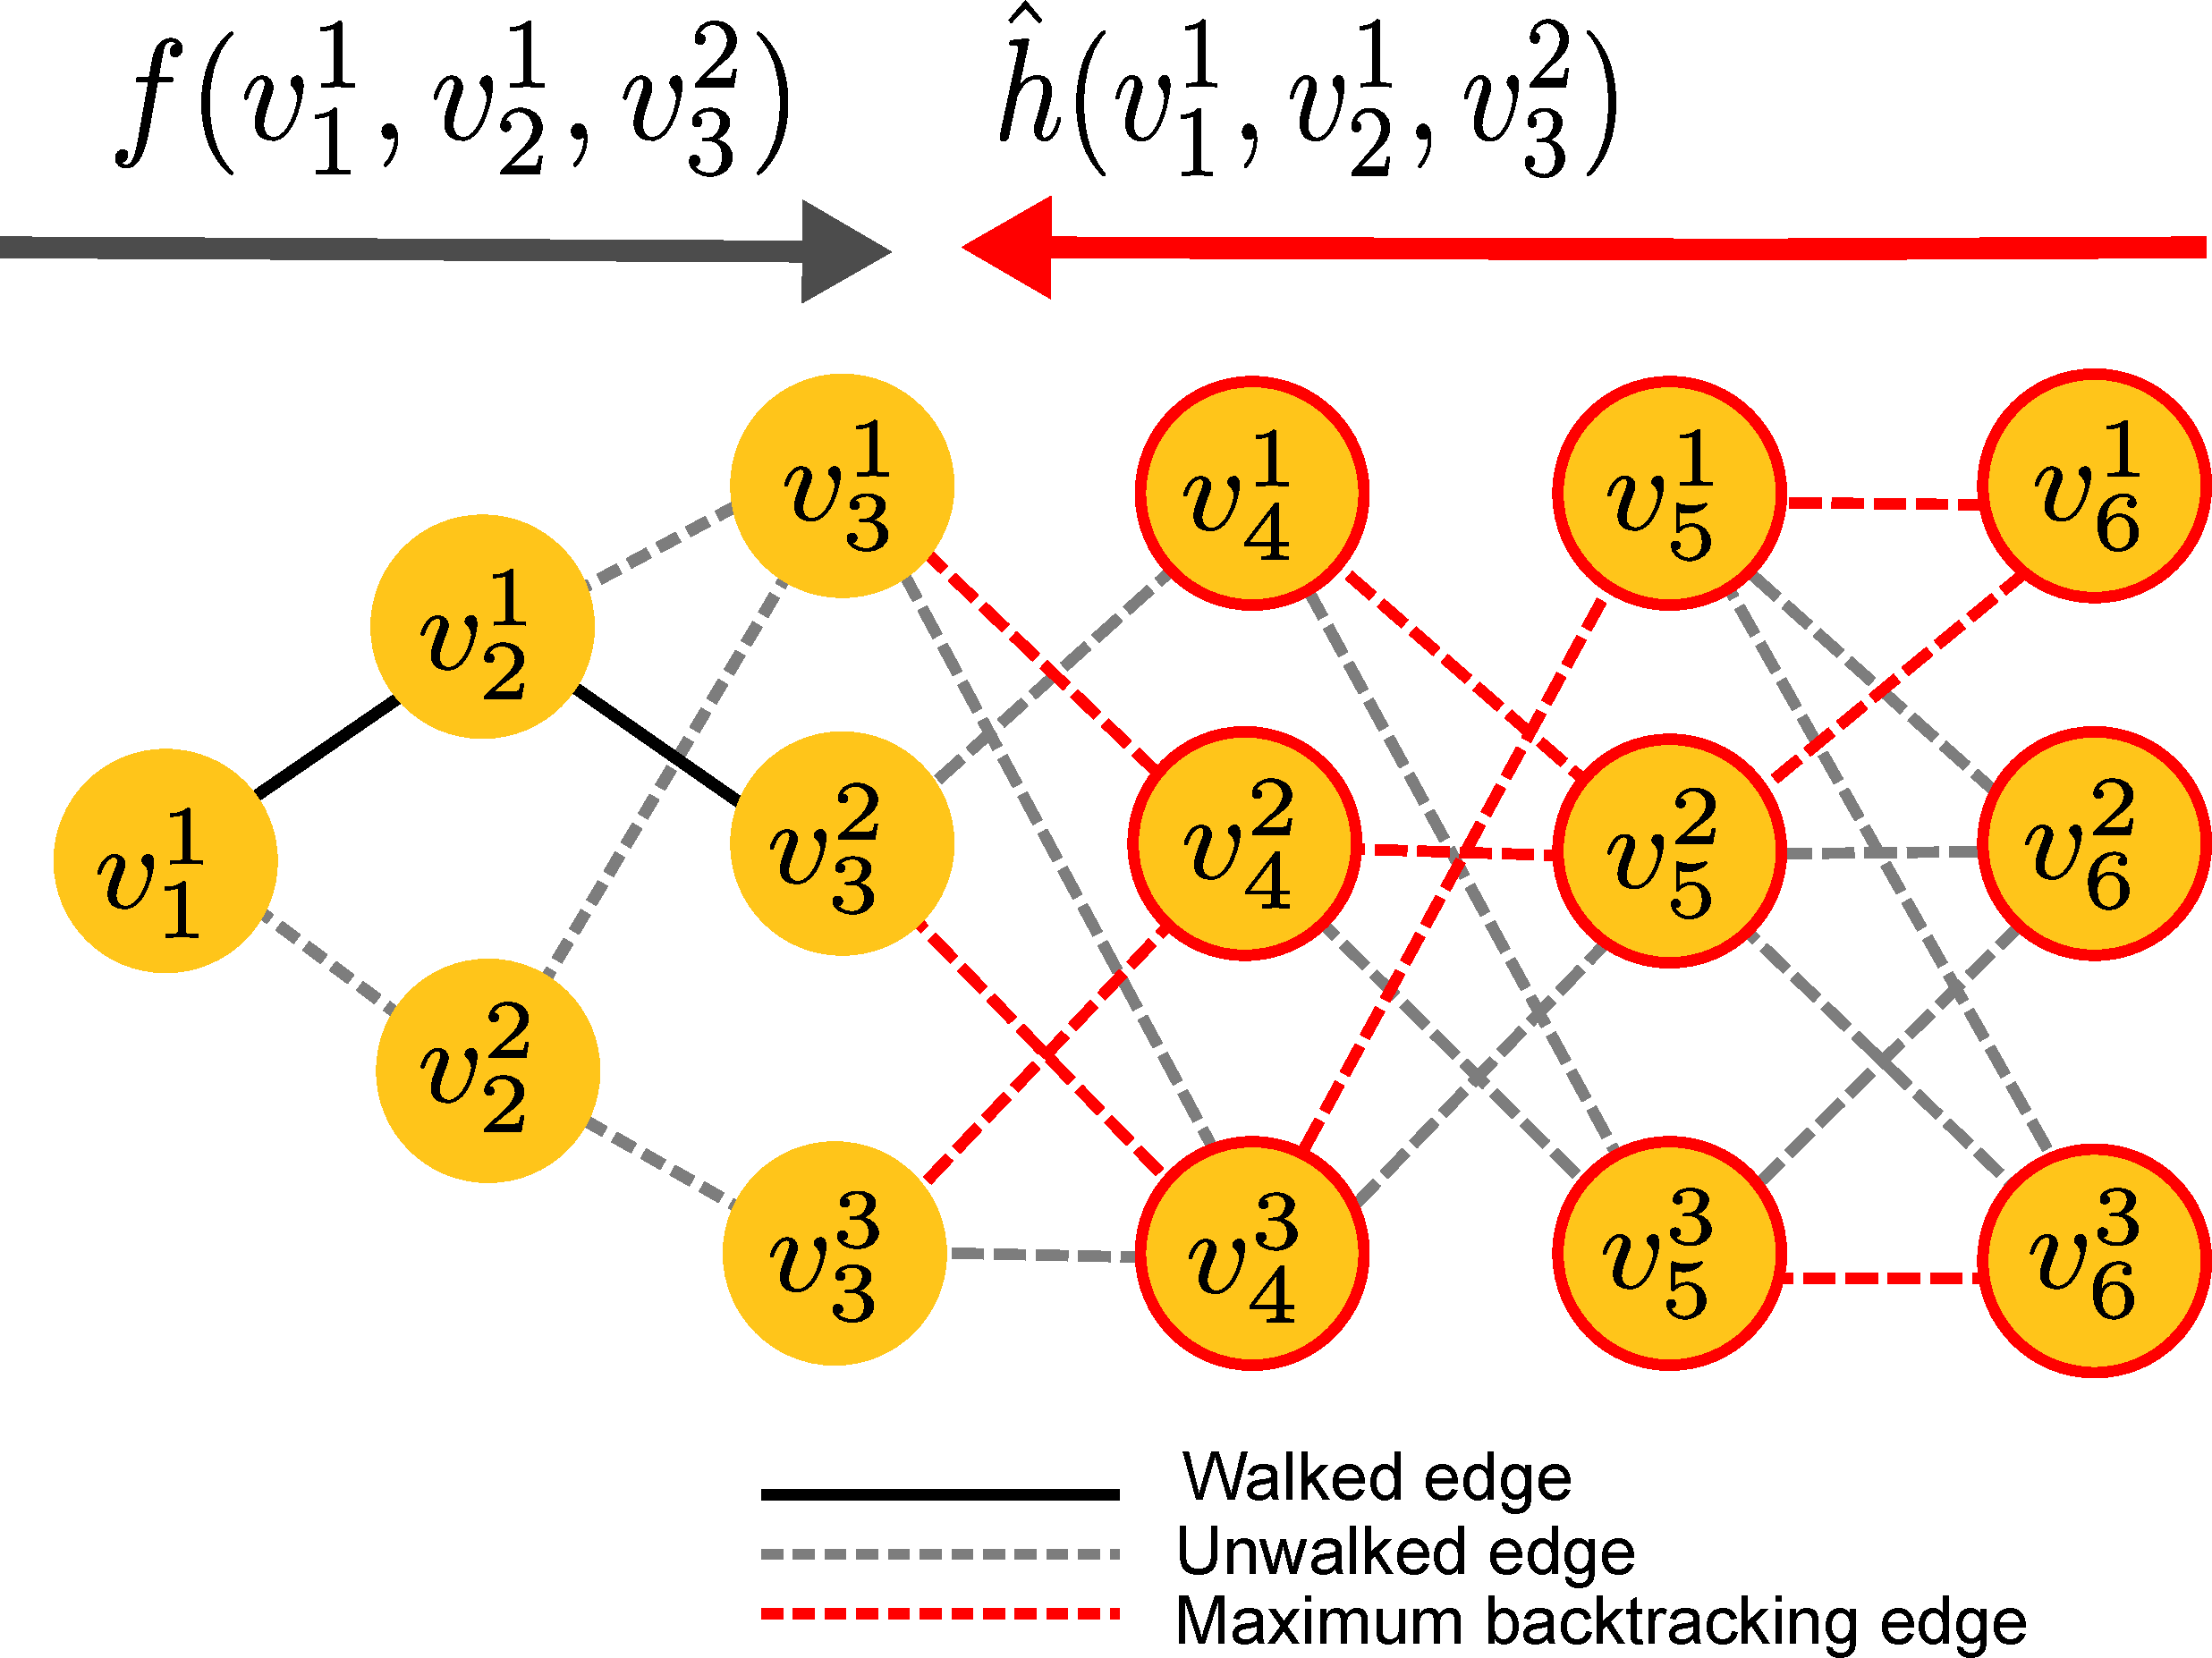
\includegraphics[width = .7\textwidth]{./figure/backtracking}
\end{figure}
\end{block}
\end{minipage}

\column{0.4\textwidth}
\begin{minipage}{\textwidth}
\begin{block}{Expanding Tree}
\begin{figure}
\centering
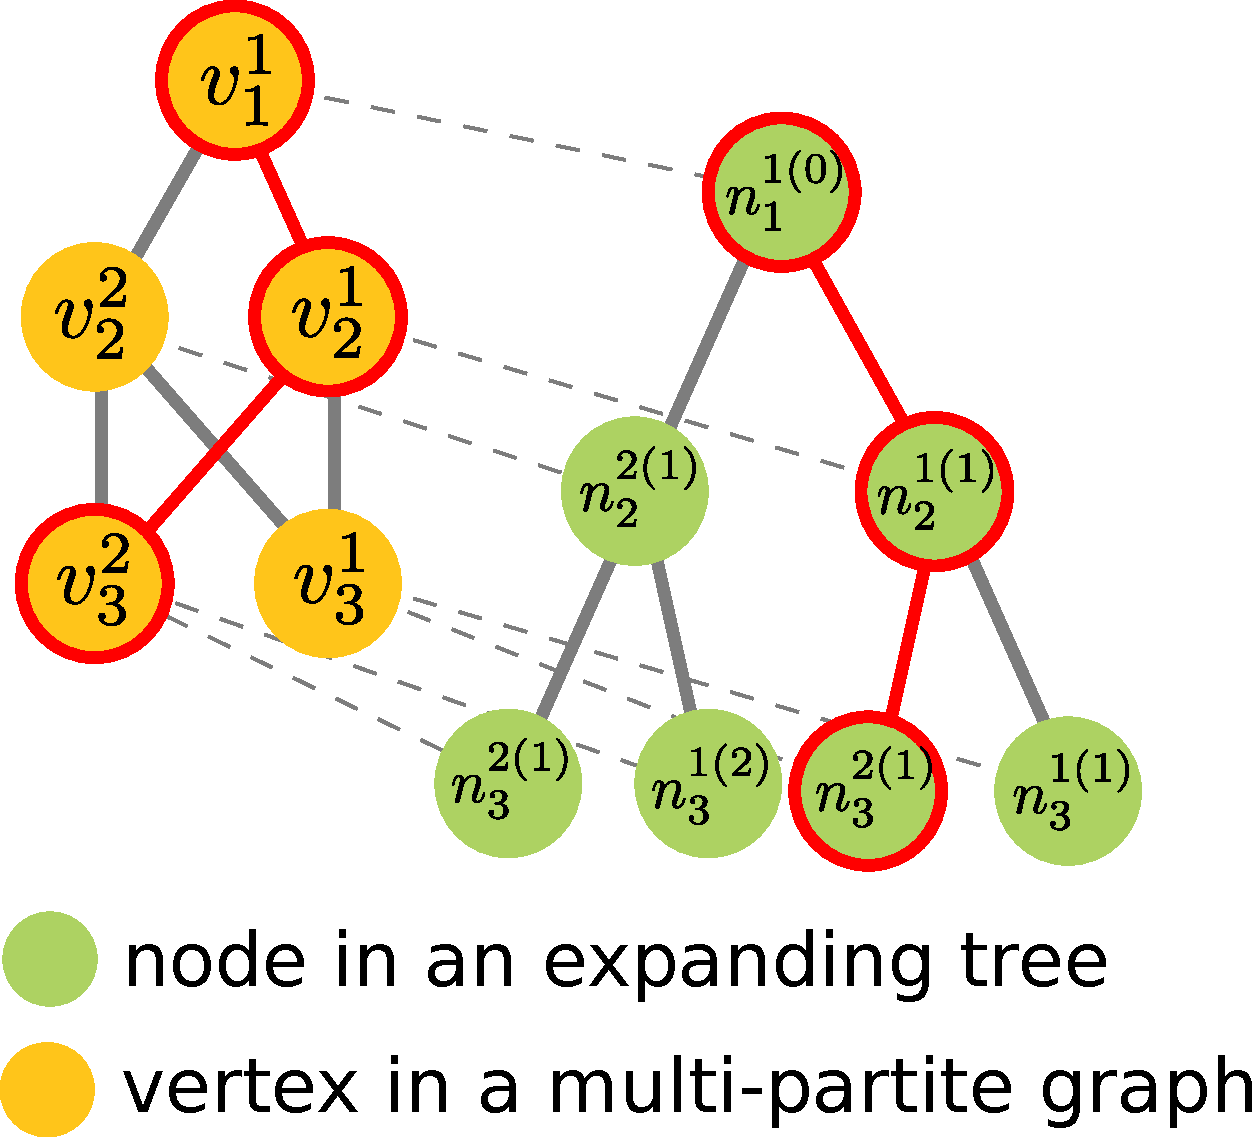
\includegraphics[width = .7\textwidth]{./figure/multipartite_expandingtree}
\end{figure}
\end{block}
\end{minipage}

\end{columns}

\centering
\begin{minipage}{.6\textwidth}
\begin{block}{Node Freeze}
\begin{figure}
\centering
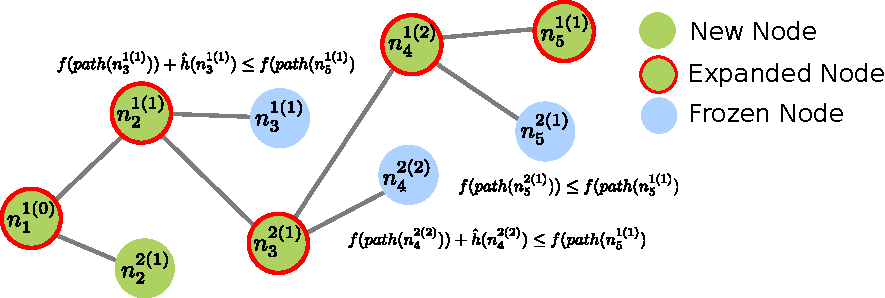
\includegraphics[width = \textwidth]{./figure/freeze_process}
\end{figure}
\end{block}
\end{minipage}

\end{frame}

\begin{frame}{Anytime Algorithm Framework}{Path-Planning with Reference Path}

\begin{figure}
\centering
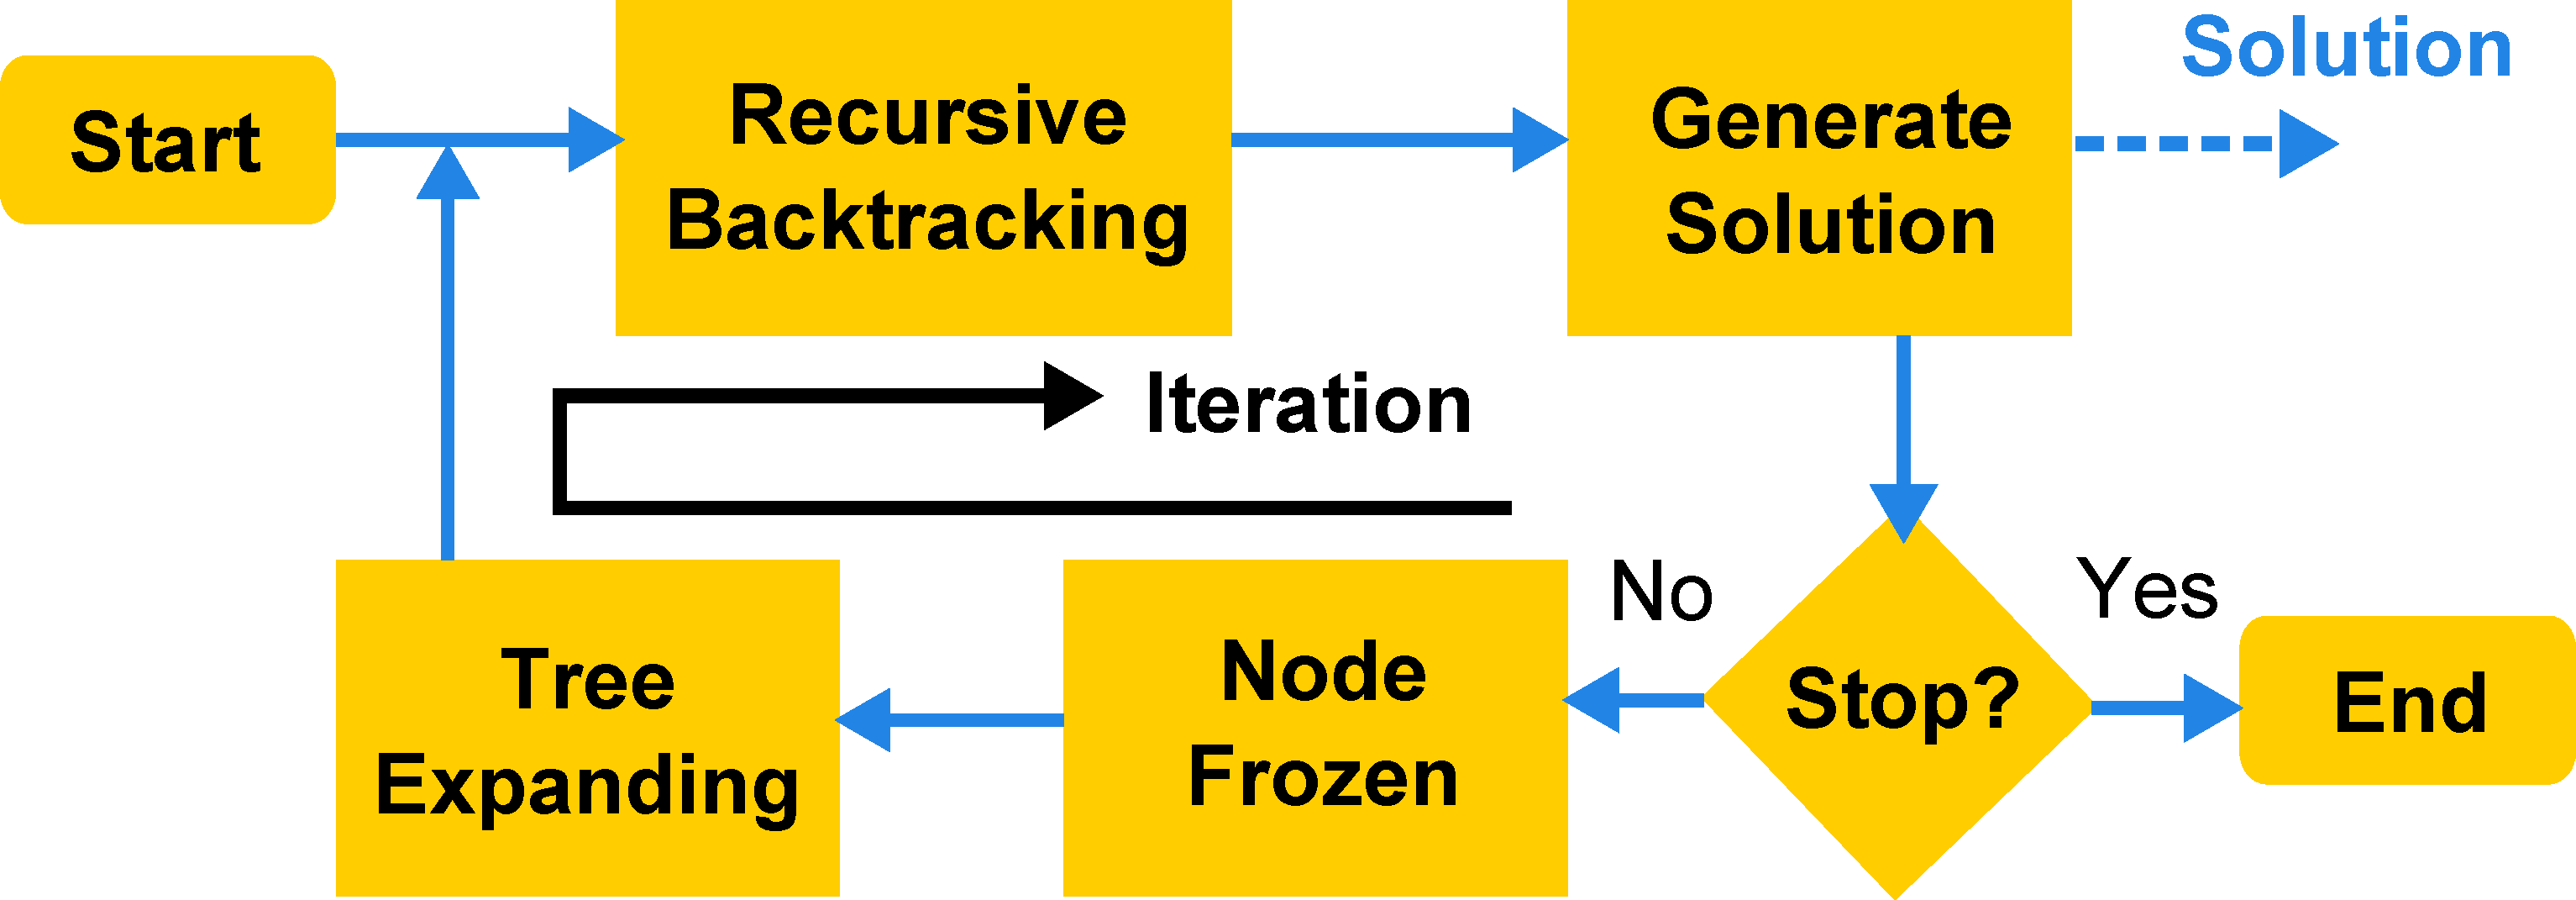
\includegraphics[width = 0.9\textwidth]{./figure/alg_flow}
\end{figure}

\end{frame}

\subsubsection{Validation}

\begin{frame}{Validation - Theoretical Analysis}{Path-Planning with Reference Path}

\begin{lemma}
Backtracking never \textcolor{red}{underestimates}
the maximum total reward, which means
\begin{equation}
\nonumber
\forall t \geq t', \hat{u}(x_{t} \mid v_{1} , \cdots , v_{t'}) \geq u(x_{t} \mid v_{1} , \cdots , v_{t'}).
\end{equation}
\end{lemma}

\begin{minipage}{\textwidth}
\begin{figure}
\centering

\includegraphics[width = 0.15\textwidth]{./figure/arrow}
\end{figure}
\end{minipage}

\begin{theorem}
The anytime algorithm framework can always find an \textcolor{red}{optimal} solution given enough time.
\end{theorem}

\end{frame}

\begin{comment}
\begin{frame}{Validation - Simulation}{Path-Planning with Reference Path}

{\bf Robot Wingman}

\begin{figure}
\centering
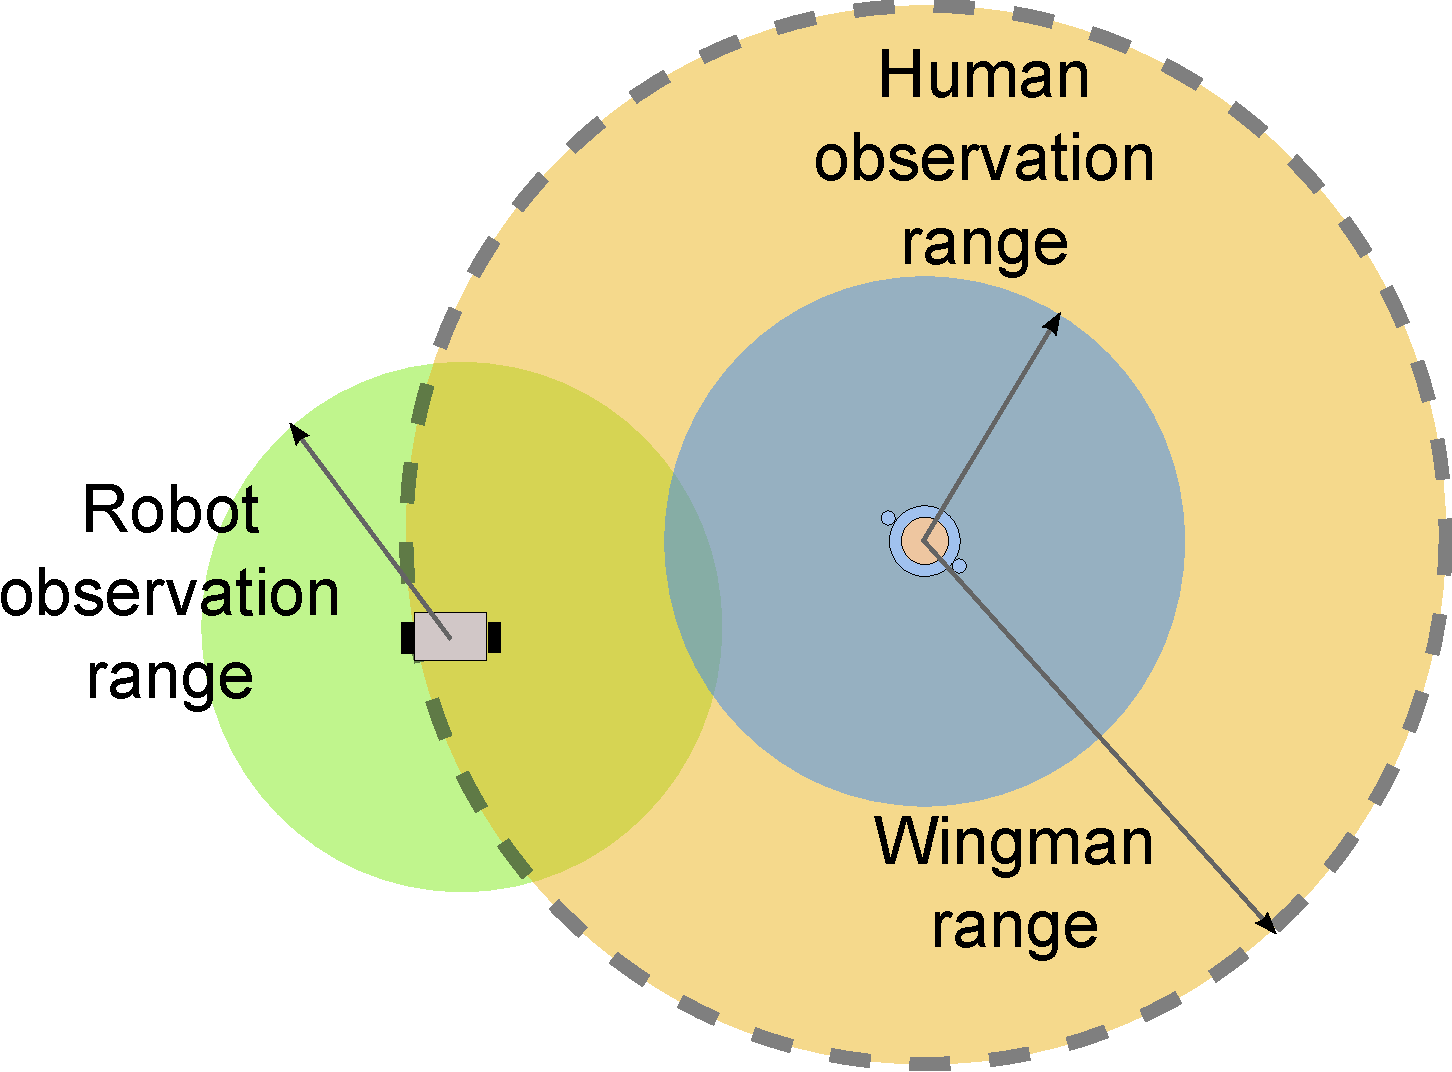
\includegraphics[width = .35\textwidth]{./figure/Wingman}
\end{figure}

\begin{columns}

\column{0.25\textwidth}
\begin{minipage}{\textwidth}
\begin{block}{Path planning}
\centering
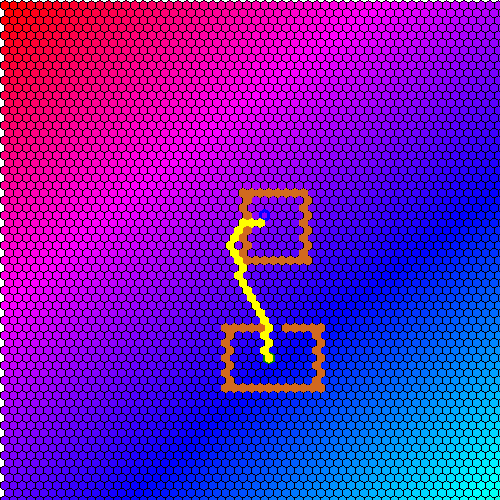
\includegraphics[width = \textwidth]{./figure/simulation/hexamap.png}
\end{block}
\end{minipage}

%\column{0.1\textwidth}
%\begin{minipage}{\textwidth}
%\centering
%
\includegraphics[width = \textwidth]{./figure/arrow2}
%\end{minipage}

\column{0.25\textwidth}
\begin{minipage}{\textwidth}
\begin{block}{Waypoints}
\centering
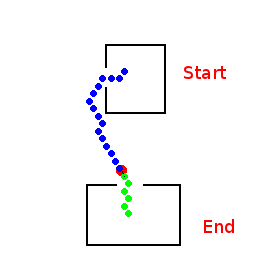
\includegraphics[width = \textwidth]{./figure/simulation/waypoint.png}
\end{block}
\end{minipage}

%\column{0.1\textwidth}
%\begin{minipage}{\textwidth}
%\centering
%
\includegraphics[width = \textwidth]{./figure/arrow2}
%\end{minipage}

\column{0.4\textwidth}
\begin{minipage}{\textwidth}
\begin{block}{Robot execution}
\centering
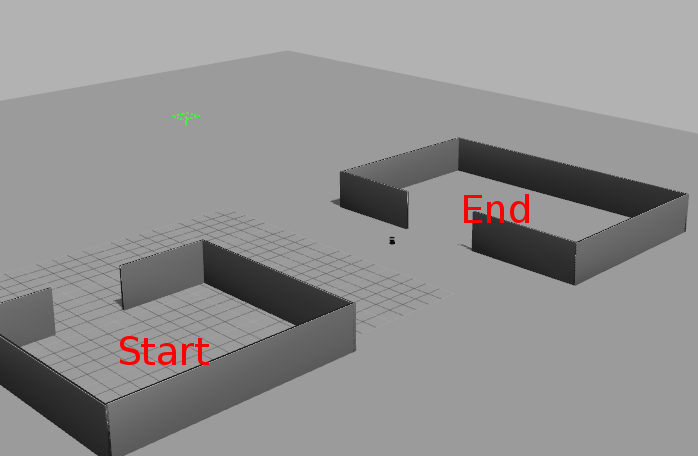
\includegraphics[width = \textwidth]{./figure/simulation/gazebo2.png}
\end{block}
\end{minipage}

\end{columns}

\end{frame}


\begin{frame}{Validation - Simulation}{Path-Planning with Reference Path}

\begin{columns}

\column{0.3\textwidth}
\begin{minipage}{\textwidth}
\begin{block}{quality of heuristic}
{\small 
\textcolor{metric-OFI}{Percentage of optimal at first iteration}
}
\end{block}
\end{minipage}

\column{0.7\textwidth}
\begin{figure}
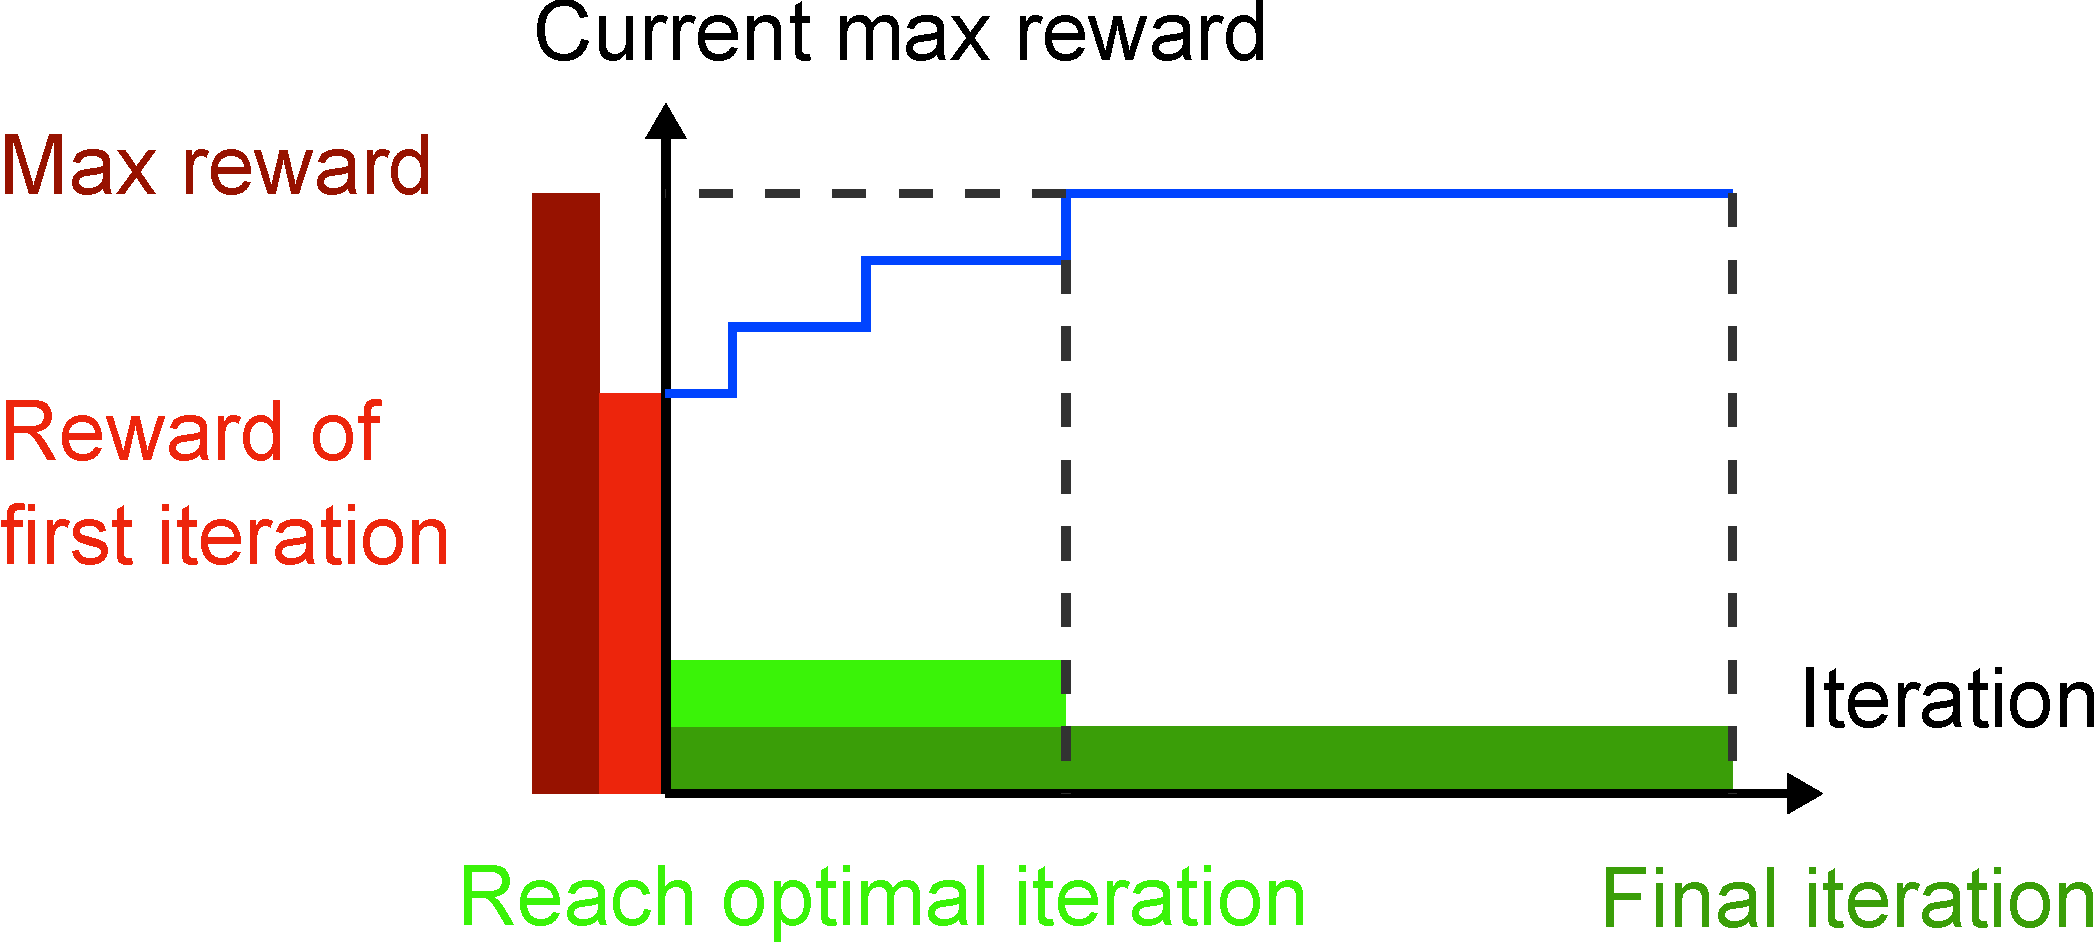
\includegraphics[width=\textwidth]{./figure/metric2}
\end{figure}

\end{columns}

\begin{columns}

\column{0.3\textwidth}

\column{0.7\textwidth}
\begin{center}
\begin{minipage}{0.43\textwidth}
\begin{block}{quality of algorithm}
{\small 
\textcolor{metric-IRO}{Number of iterations to reach optimal (normalized)}
}
\end{block}
\end{minipage}
\end{center}

\end{columns}

\end{frame}
\end{comment}
\begin{frame}{Validation - Simulation}{Path-Planning with Reference Path}

\begin{columns}[t]

\column{0.32\textwidth}
\begin{block}{Heuristic}
\begin{itemize}
\item greedy heuristic 
\item backtracking heuristic
\end{itemize}
\end{block}

\column{0.32\textwidth}
\begin{block}{Environment}
\begin{itemize}
\item Uniform
\item Random	
\item Multi-Modal
\end{itemize}
\end{block}

\column{0.32\textwidth}
\begin{block}{Reference Paths}
\begin{itemize}
\item Line
\item Spiral
\item Lawn-mower
\item Arc
\item Loitering
\end{itemize}
\end{block}

\end{columns}

\end{frame}



